%%%%%%%%%%%%%%%%%%%%%%%%%%%%%%%%%%%%%%%%%%%%%%%%%%%%%%%%%%%%%%%%%%%%%%%%%%%%%%%
% Memorial para concurso público de Professor Doutor na USP.
%
% Formatação inspirada em:
% * https://tug.org/pracjourn/2008-1/mori/mori.pdf
% * https://github.com/santisoler/phd-thesis
% * https://github.com/compgeolab/dissertation-template
%%%%%%%%%%%%%%%%%%%%%%%%%%%%%%%%%%%%%%%%%%%%%%%%%%%%%%%%%%%%%%%%%%%%%%%%%%%%%%%

%%%%%%%%%%%%%%%%%%%%%%%%%%%%%%%%%%%%%%%%%%%%%%%%%%%%%%%%%%%%%%%%%%%%%%%%%%%%%%%
% Set a class and import packages
\documentclass[10pt,a4paper,oneside]{book}

% Variables
\newcommand{\Year}{2022}
\newcommand{\Author}{Leonardo Uieda}
\newcommand{\Title}{Memorial de \Author{} para concurso público - Professor Doutor em Geofísica - IAG/USP}
\newcommand{\Email}{Leonardo.Uieda@liverpool.ac.uk}
\newcommand{\EmailPersonal}{leouieda@gmail.com}
\newcommand{\ORCID}{0000-0001-6123-9515}
\newcommand{\ResearcherID}{G-3258-2012}
\newcommand{\GoogleScholar}{qfmPrUEAAAAJ}
\newcommand{\Lattes}{8939551682050504}

% Variables for easier typing of some names
\newcommand{\UHM}{University of Hawai`i at M\={a}noa}
\newcommand{\UERJ}{Universidade do Estado do Rio de Janeiro}

% Names for citing coauthors
\newcommand{\Me}{\textbf{Uieda, L}}
\newcommand{\Val}{Barbosa, VCF}
\newcommand{\Bi}{Oliveira Jr, VC}
\newcommand{\Paul}{Wessel, P}
\newcommand{\Joaquim}{Luis, J}
\newcommand{\Remko}{Scharroo, R}
\newcommand{\Florian}{Wobbe, F}
\newcommand{\Walter}{Smith, WHF}
\newcommand{\Dongdong}{Tian, D}
\newcommand{\Bridget}{Smith-Konter, B}
\newcommand{\Eric}{Xu, X}
\newcommand{\David}{Sandwell, DT}
\newcommand{\Carla}{Braitenberg, C}
\newcommand{\Naomi}{Ussami, N}
\newcommand{\Manoel}{D'Agrella-Filho, MS}
\newcommand{\JB}{Silva, JBC}
\newcommand{\Dai}{Sales, DP}
\newcommand{\Figura}{Melo, FF}
\newcommand{\Dio}{Carlos, DU}
\newcommand{\BragaVale}{Braga, MA}
\newcommand{\YLi}{Li, Y}
\newcommand{\Angeli}{Angeli, G}
\newcommand{\Peres}{Peres, G}
\newcommand{\Everton}{Bomfim, EP}
\newcommand{\Eder}{Molina, E}
\newcommand{\Gomes}{Gomes, AAS}
\newcommand{\Santiago}{Soler, SR}
\newcommand{\Agustina}{Pesce, A}
\newcommand{\Gimenez}{Gimenez, ME}
\newcommand{\Kristoffer}{Hallam, KAT}
\newcommand{\Guangdong}{Zhao, G}
\newcommand{\Bo}{Chen, B}
\newcommand{\JLiu}{Liu, J}
\newcommand{\LChen}{Chen, L}
\newcommand{\RGuo}{Guo, R}
\newcommand{\MKaban}{Kaban, MK}
\newcommand{\Lindsey}{Heagy, LJ}
\newcommand{\Lion}{Krischer, L}
\newcommand{\Rene}{Gassmoeller, R}
\newcommand{\Bane}{Sullivan, CB}
\newcommand{\Jens}{Klump, JF}
\newcommand{\LBarba}{Barba, LA}
\newcommand{\JBazan}{Bazan, J}
\newcommand{\JBrown}{Brown, J}
\newcommand{\RGuimera}{Guimera, RV}
\newcommand{\MGymrek}{Gymrek, M}
\newcommand{\AHanna}{Alex Hanna}
\newcommand{\KHuff}{Huff, KD}
\newcommand{\DKatz}{Katz, DS}
\newcommand{\CMadan}{Madan, CR}
\newcommand{\KMoerman}{Moerman, KM}
\newcommand{\KNiemeyer}{Niemeyer, KE}
\newcommand{\JPoulson}{Poulson, JL}
\newcommand{\PPrins}{Prins, P}
\newcommand{\KRam}{Ram, K}
\newcommand{\ARokem}{Rokem, A}
\newcommand{\Arfon}{Smith, AM}
\newcommand{\GThiruvathukal}{Thiruvathukal, GK}
\newcommand{\KThyng}{Thyng, KM}
\newcommand{\BWilson}{Wilson, BE}
\newcommand{\Yehudi}{Yehudi, Y}
\newcommand{\Remi}{Rampin, R}
\newcommand{\Hugo}{van Kemenade, H}
\newcommand{\MattTurk}{Turk, M}
\newcommand{\Shapero}{Shapero, D}
\newcommand{\Anderson}{Banihirwe, A}
\newcommand{\Leeman}{Leeman, J}
\newcommand{\JEbbing}{Ebbing, J}
\newcommand{\AGuy}{Guy, A}
\newcommand{\JFarquharson}{Farquharson, J}
\newcommand{\AKushnir}{Kushnir, A}
\newcommand{\FWadsworth}{Wadsworth, F}
\newcommand{\LPerozzi}{Perozzi, L}
\newcommand{\MWieczorek}{Wieczorek, MA}
\newcommand{\LLi}{Li, L}
\newcommand{\Ricardo}{Trindade, RIF}

\usepackage[utf8]{inputenc}
\usepackage[T1]{fontenc}
\usepackage[brazil]{babel}
\usepackage{geometry}
\usepackage{graphicx}
\usepackage{amssymb}
\usepackage{amsmath}
\usepackage{hyperref}
% create fancy headers
\usepackage{fancyhdr}
% commands for managing dates and its formats
\usepackage{datetime2}
% improved urls with proper hyphenation
\usepackage{xurl}
% Import enumitem to customize descriptions in license.tex
\usepackage{enumitem}
% Tweak the look of captions
\usepackage{caption}
% To control the style of section titles
\usepackage{titlesec}
% Add the bibliography to the table of contents
\usepackage[nottoc,chapter]{tocbibind}
\usepackage[round,authoryear,sort]{natbib}
% show dois as links on references
\usepackage{doi}
% Icon fonts (requires using xelatex or luatex)
\usepackage{fontawesome5}
\usepackage{academicons}
\usepackage{fontspec}
% Set fonts (requires compilation with xelatex)
\usepackage{fontspec}
\usepackage{microtype}
% To make fancy text boxes
\usepackage{xcolor}
\usepackage[framemethod=tikz]{mdframed}
% For fancy and multipage tables
\usepackage{tabularx}
\usepackage{ltablex}
% To define custom environments
\usepackage{environ}
\usepackage{setspace}
% Reference sections by name
\usepackage{nameref}
% Better handling of footnotes inside summary boxes
\usepackage{footmisc}
%%%%%%%%%%%%%%%%%%%%%%%%%%%%%%%%%%%%%%%%%%%%%%%%%%%%%%%%%%%%%%%%%%%%%%%%%%%%%%%

%%%%%%%%%%%%%%%%%%%%%%%%%%%%%%%%%%%%%%%%%%%%%%%%%%%%%%%%%%%%%%%%%%%%%%%%%%%%%%%
% Configuration of the document

\geometry{%
  left=30mm,
  right=30mm,
  top=20mm,
  bottom=15mm,
  headsep=5mm,
  headheight=5mm,
  footskip=10mm,
  includehead=true,
  includefoot=true
}

\setmainfont[%
  Path=fonts/notoserif/,
  UprightFont=NotoSerif-Regular,
  BoldFont=NotoSerif-Bold,
  ItalicFont=NotoSerif-Italic,
  Extension=.ttf
]{NotoSerif}

% Increase the line spacing
\SetSinglespace{1.2}
\onehalfspacing

% Padding between the first figure and the chapter title
\newcommand{\HeroFigPad}{\vspace{-1cm}}

% Add a link to a DOI
\newcommand{\DOI}[1]{\url{https://doi.org/#1}}

% Add a link to a GitHub repository
\newcommand{\GitHub}[1]{\faGithub{} Código: \url{https://github.com/#1}}

% Add a link to a YouTube video
\newcommand{\YouTube}[1]{\faYoutube{} Vídeo: \url{https://youtu.be/#1}}

% Add a link to a supplementary data
\newcommand{\Data}[1]{\faChartBar{} Dados: \url{https://doi.org/#1}}

% Add a link to a preprint
\newcommand{\Preprint}[1]{\faLockOpen{} Preprint: \url{https://doi.org/#1}}

% Add a link without the HTTPS part
\newcommand{\prettyhref}[1]{\url{#1}}

% Define custom colors
\definecolor{lu_gray}{gray}{0.98}
\definecolor{lu_darkgray}{gray}{0.3}
\definecolor{lu_blue}{RGB}{32, 96, 194}
\definecolor{lu_lightblue}{RGB}{238, 245, 250}
\definecolor{lu_yellow}{RGB}{255, 193, 7}
\definecolor{lu_lightyellow}{RGB}{255, 249, 230}

% Customize how Chapter headings are displayed
\titleformat{\chapter}[display]{\normalfont}{\large Capítulo \thechapter}{0pt}{\huge}[\titlerule]
\titlespacing*{\chapter}{0pt}{-40pt}{40pt}

% Set the spacing between bibliography entries (requires natbib)
\setlength{\bibsep}{0pt}

% Configure captions
\captionsetup{labelfont=bf,font={small,color=lu_darkgray},skip=0pt}

% Define a fancy text box
\mdfdefinestyle{summarybox}{%
  leftline=true,
  rightline=false,
  topline=false,
  bottomline=false,
  linewidth=4pt,
  linecolor=lu_blue,
  frametitlefont=\bfseries\color{black},
  frametitlebackgroundcolor=lu_lightblue,
  frametitleaboveskip=10pt,
  frametitlebelowskip=10pt,
  frametitlerule=true,
  frametitlerulewidth=1pt,
  backgroundcolor=lu_gray,
  innertopmargin=10pt,
  innerbottommargin=15pt,
  innerleftmargin=15pt,
  innerrightmargin=15pt,
}
\newmdenv[style=summarybox]{summarybox}
\mdfdefinestyle{subsummarybox}{%
  leftline=true,
  rightline=false,
  topline=false,
  bottomline=false,
  linewidth=4pt,
  linecolor=lu_yellow,
  frametitlefont=\bfseries\color{black},
  frametitlebackgroundcolor=lu_lightyellow,
  frametitleaboveskip=10pt,
  frametitlebelowskip=10pt,
  frametitlerule=true,
  frametitlerulewidth=1pt,
  backgroundcolor=lu_gray,
  innertopmargin=10pt,
  innerbottommargin=15pt,
  innerleftmargin=15pt,
  innerrightmargin=15pt,
}
\newmdenv[style=subsummarybox]{subsummarybox}

% Define something like an fa-ul and a date list
\NewEnviron{fa-ul}{%
  \vspace{-0.4cm}
  \renewcommand{\arraystretch}{1.25}
  \begin{tabularx}{\linewidth}{@{}p{0.06\linewidth}@{}@{}p{0.94\linewidth}@{}}
    \BODY
  \end{tabularx}%
}
\NewEnviron{datelist}{%
  \vspace{-0.4cm}
  \renewcommand{\arraystretch}{1.25}
  \begin{tabularx}{\linewidth}{@{}p{0.15\linewidth}@{}@{}p{0.85\linewidth}@{}}
    \BODY
  \end{tabularx}%
}
\NewEnviron{paperlist}{%
  \vspace{-0.4cm}
  \renewcommand{\arraystretch}{1.25}
  \begin{tabularx}{\linewidth}{@{}p{0.08\linewidth}@{}@{}p{0.92\linewidth}@{}}
    \BODY
  \end{tabularx}%
}
\NewEnviron{courselist}{%
  \vspace{-0.4cm}
  \renewcommand{\arraystretch}{1.25}
  \begin{tabularx}{\linewidth}{@{}p{0.15\linewidth}@{}@{}p{0.85\linewidth}@{}}
    \BODY
  \end{tabularx}
}

% Configure hyperref and add PDF metadata
\hypersetup{
    colorlinks,
    allcolors=lu_blue,
    pdftitle={\Title},
    pdfauthor={\Author},
    pdftex,
    breaklinks=true,
}

% make urls use the same font as every other text
\urlstyle{same}

% Prevent footnotes from being broken into multiple pages
\interfootnotelinepenalty=10000

% Configure headers and footers
\fancyhf{}
\lhead{\fontsize{9pt}{0}\selectfont\itshape \nouppercase\leftmark}
\chead{}
\rhead{\fontsize{9pt}{0}\selectfont \thepage}
\cfoot{}
\renewcommand{\headrulewidth}{0.3pt}
%%%%%%%%%%%%%%%%%%%%%%%%%%%%%%%%%%%%%%%%%%%%%%%%%%%%%%%%%%%%%%%%%%%%%%%%%%%%%%%

%%%%%%%%%%%%%%%%%%%%%%%%%%%%%%%%%%%%%%%%%%%%%%%%%%%%%%%%%%%%%%%%%%%%%%%%%%%%%%%
\begin{document}

\pagestyle{plain}
\frontmatter

\begin{titlepage}
  \begin{center}
    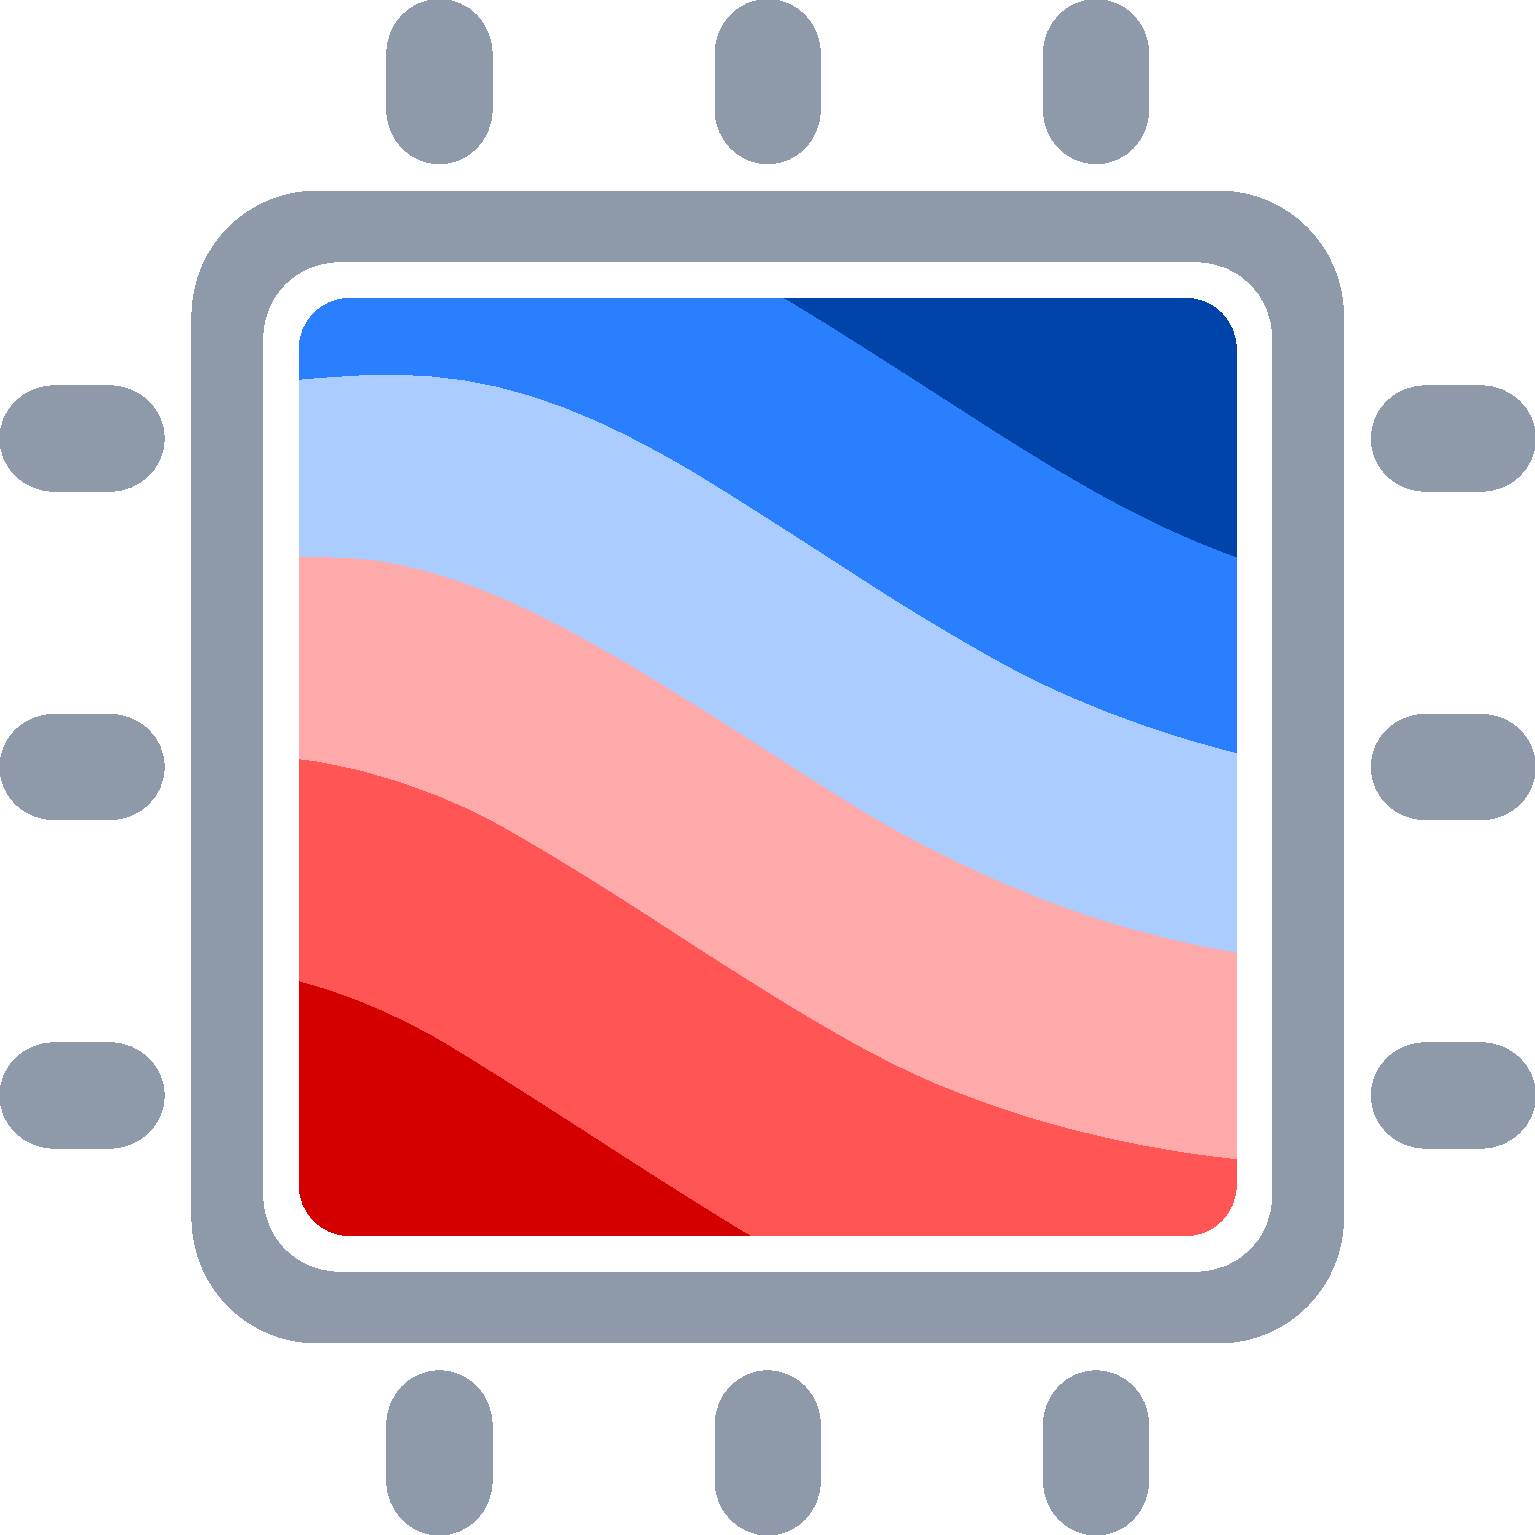
\includegraphics[height=2cm]{images/logo.pdf}
    \vspace{2cm}

    MEMORIAL PARA CONCURSO PÚBLICO

    PROFESSOR DOUTOR (RDIDP) EM MÉTODOS POTENCIAIS

    UNIVERSIDADE DE SÃO PAULO
    \vspace{5cm}

    \textbf{\LARGE \MakeUppercase{\Author{}}}
    \vspace{5cm}

    {\small
      Apresentado para concurso público de títulos e provas para cargo de

      Professor Doutor junto ao Departamento de Geofísica do

      Instituto de Astronomia, Geofísica e Ciências Atmosféricas da

      Universidade de São Paulo.
      \vspace{1cm}

      Edital ATAc-IAG/044/2022
    }
    \vfill

    \Year{}
  \end{center}
\end{titlepage}

%==============================================================================
\chapter*{Resumo}

Possuo Bacharelado em Geofísica pela Universidade de São Paulo e Mestrado
e Doutorado em Geofísica pelo Observatório Nacional.
Ao longo da minha formação e carreira, passei por seis instituições de ensino
superior em quarto países diferentes.
Trabalhei como Professor Assistente na \UERJ{},
Professor Visitante na \UHM{} e atualmente sou Lecturer (equivalente a
Professor Doutor) na University of Liverpool.
Ministrei 10 disciplinas diferentes a nível de graduação e 17 cursos de curta
duração abrangendo uma gama de tópicos da geofísica, geologia e programação.
Sou autor de 16 artigos científicos que agregam mais de 1700
citações\footnote{Segundo Google Scholar em 27/12/2022: \url{https://scholar.google.com/citations?user=qfmPrUEAAAAJ}}.
Atuo na área de ciência aberta e reprodutibilidade desde meu primeiro artigo
publicado em 2012 durante meu Mestrado.
Desenvolvo diversos projetos de software livre para ciência que atraem centenas
de milhares de downloads
mensais\footnote{Por exemplo, o software \href{https://github.com/fatiando/pooch}{Pooch}:
\url{https://pypistats.org/packages/pooch}}.
Sou reconhecido por minha expertise em Geociências, desenvolvimento de software
e ciência aberta, tendo servido como editor do
\href{https://joss.theoj.org/}{Journal of Open Source Software} e na
coordenação das organizações internacionais
\href{https://eartharxiv.org/}{EarthArXiv},
\href{https://www.pyopensci.org/}{pyOpenSci}
e \href{https://softwareunderground.org}{Software Underground}.

Este memorial apresenta minha formação e atuação profissional, incluindo
reflexões sobre os fatores que me trouxeram até onde estou e as lições que
aprendi ao longo do caminho.
Além disso, o memorial também relata meus planos futuros para meu
desenvolvimento profissional e a minha motivação para retornar à Universidade
de São Paulo, onde iniciei minha trajetória 19 anos atrás.

\begin{figure}[pb]
  %\vspace{1cm}
  \begin{center}
    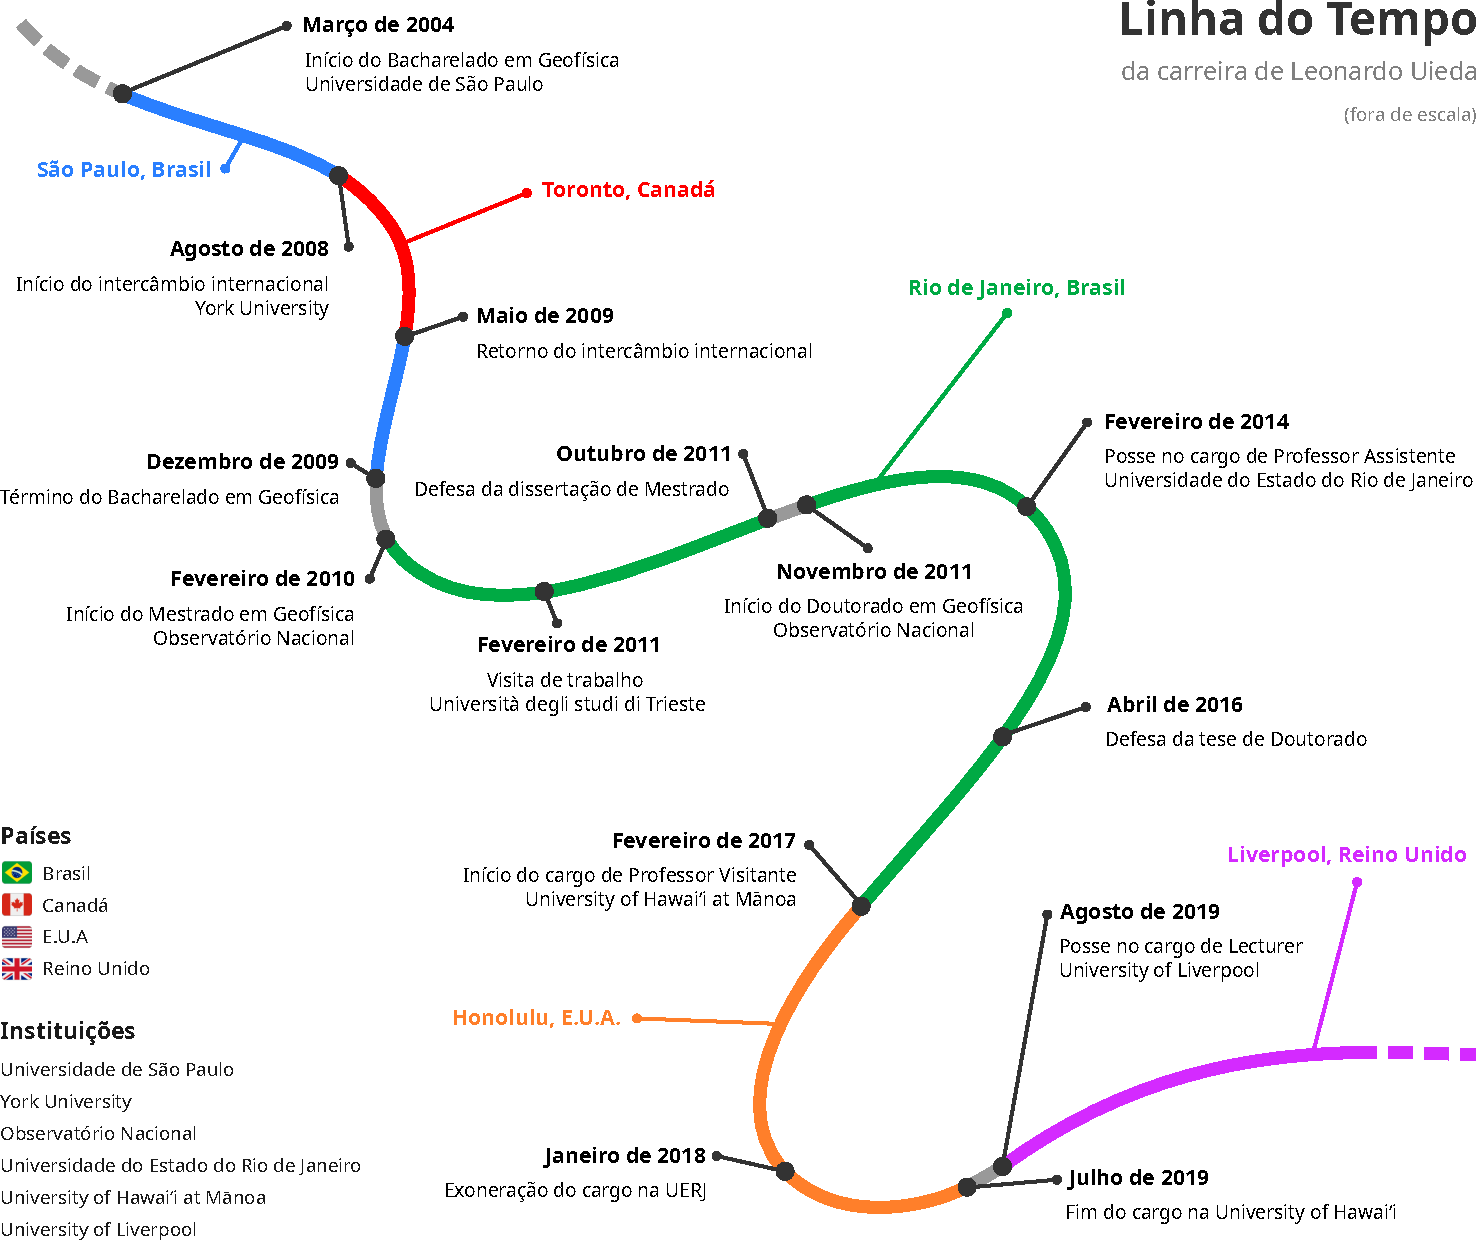
\includegraphics[width=\textwidth]{images/timeline.pdf}
  \end{center}
  \caption*{
    Linha do tempo (fora de escala) resumindo minha trajetória acadêmica, desde
    o início do meu curso de Bacharelado em Geofísica na Universidade de São
    Paulo em 2004 até meu cargo de Lecturer na University of Liverpool de 2019
    até o presente.
  }
\end{figure}

%==============================================================================
\tableofcontents

\mainmatter
\pagestyle{fancy}

%==============================================================================
\chapter{Introdução}

\begin{figure}[h]
  \HeroFigPad
  \begin{center}
    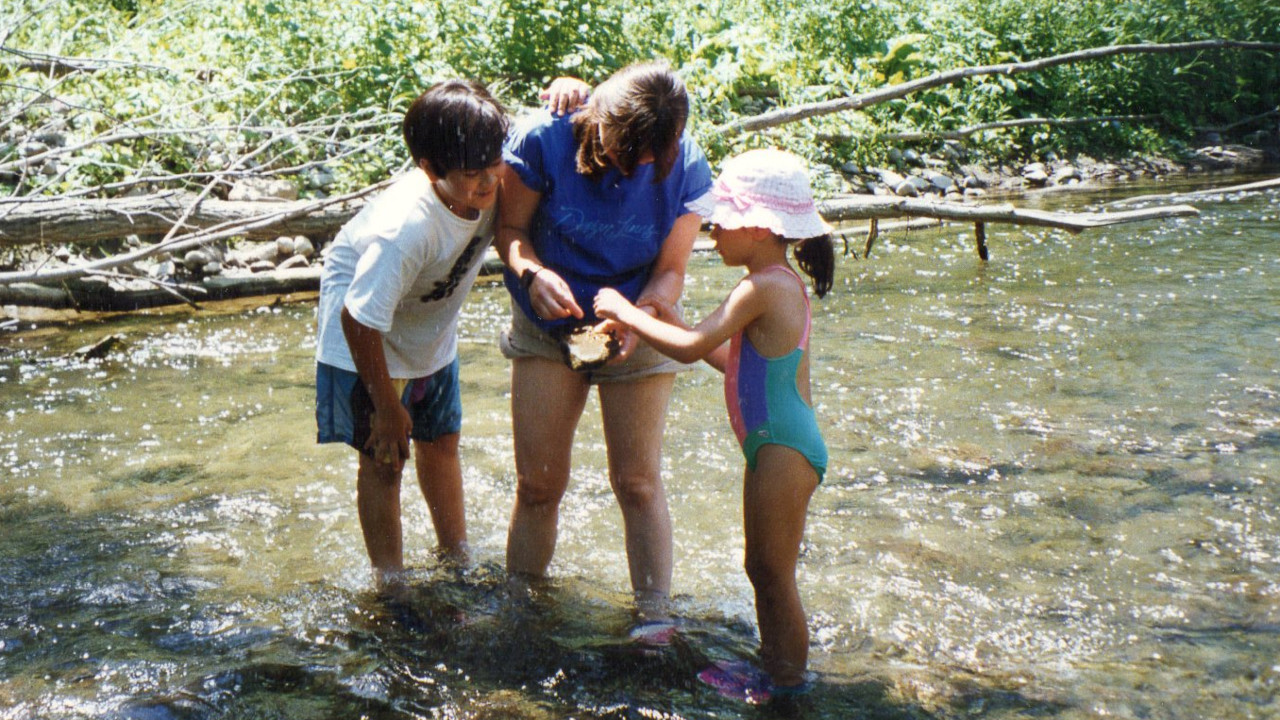
\includegraphics[width=\textwidth]{images/1997-06-ithaca-creek.jpg}
  \end{center}
  \caption{
    Minha mãe mostrando para mim e minha irmã caçula o lado inferior de uma
    pedra em um riacho, provavelmente contendo invertebrados aquáticos.
    Foto de Junho de 1997, tirada no interior do estado de Nova York, E.U.A.,
    durante o pós-doutorado de meus pais na
    \href{https://www.cornell.edu/}{Cornell University}.
  }
  \label{fig_riacho}
\end{figure}
\begin{summarybox}[frametitle=\faInfoCircle{}\quad Informações para contato]
  \begin{fa-ul}
    \faEnvelope & email profissional: \href{mailto:\Email}{\Email} \\
    \faEnvelope & email pessoal: \href{mailto:\EmailPersonal}{\EmailPersonal} \\
    \aiOrcid & ORCID: \href{https://orcid.org/\ORCID}{\ORCID} \\
    \aiLattes & Currículo Lattes: \url{https://lattes.cnpq.br/\Lattes} \\
    \aiPublonsSquare & ResearcherID: \href{https://www.webofscience.com/wos/author/rid/\ResearcherID}{\ResearcherID} \\
    \faUser & Página pessoal: \url{https://www.leouieda.com} \\
    \faUsers & Grupo de pesquisa: \url{https://www.compgeolab.org}
  \end{fa-ul}
\end{summarybox}

Este memorial apresenta uma análise reflexiva sobre os principais temas de minha
carreira acadêmica: minha formação, minhas linhas de pesquisa, minhas atividades
de ensino e extensão e meus esforços para tornar a ciência feita em nossa
disciplina mais aberta, reprodutível e reutilizável.
Ao buscar a fonte de vários dos princípios que me guiam hoje em dia, percebi
que o ponto mais adequado para começar seria com uma análise das influências
que tive durante minha criação.

\section{Influências durante a infância e a adolescência}

Meu primeiro contato com a ciência foi através de meus pais,
\href{https://orcid.org/0000-0002-6078-1342}{Virginia Sanches Uieda} e
\href{https://orcid.org/0000-0002-4177-3339}{Wilson Uieda},
ambos professores do Instituto de Biociências da Universidade Estadual Paulista
Júlio de Mesquita Filho (UNESP) de Botucatu, São Paulo.
Eles rotineiramente incluíam minhas duas irmãs e eu em suas atividades como
docentes da UNESP, o que nos proporcionou oportunidades de aprendizagem únicas
e que foram particularmente influentes na minha formação.
Tenho memórias marcantes de coletar peixes e invertebrados aquáticos com minha
mãe (figura~\ref{fig_riacho}), fotografar morcegos do gênero
\href{https://pt.wikipedia.org/wiki/Artibeus}{\textit{Artibeus}} se alimentando
dos frutos do chapéu-de-sol com meu pai, observar minha mãe corrigindo provas
de zoologia de vertebrados e tentar acertar mais questões que seus alunos,
alimentar os morcegos
\href{https://pt.wikipedia.org/wiki/Desmodus_rotundus}{\textit{Desmodus rotundus}}
que meu pai mantinha em cativeiro com cubos de sangue bovino congelado nos
finais de semana, acompanhar minha mãe na disciplina de campo sobre cetáceos
onde pudemos interagir diretamente com botos-cinza
(\href{https://pt.wikipedia.org/wiki/Sotalia_guianensis}{\textit{Sotalia guianensis}})
em seu habitat natural.

A curiosidade, a dedicação e a ética dos meus pais formaram a base da minha
posição a respeito da ciência e do que significa ser um educador de qualidade.
Essa base e o todo apoio que recebi de meus pais foram fundamentais para
conquistar tudo o que consegui até hoje (i.e., o conteúdo desse memorial).

\section{Reflexão sobre vantagens e privilégios}

Esse memorial representa todas as minhas conquistas ao longo da minha carreira.
Dedicação, esforço e talento (i.e., mérito) foram certamente importantes para
meu sucesso profissional.
Porém, seria muito ingênuo de minha parte assumir que esses foram os únicos
fatores que influenciaram minha trajetória.
Por isso acho importante refletir sobre as vantagens e privilégios que tive
sobre meus contemporâneos para dar contexto ao resto do memorial.

Primeiramente, sou homem, heterossexual, cisgênero e de etnia mista branca
europeia e norte asiática.
A junção desses fatores significa que, por nenhum mérito próprio, tive que
superar um número consideravelmente menor de barreiras ao longo de minha
carreira que outras pessoas.
Fui criado por pais dedicados e com imenso suporte de toda minha família
estendida.
Minha família é de classe média alta e tive acesso a educação privada em boas
escolas.
Ao contrário de alguns dos meus colegas do curso de graduação, não tive que
trabalhar para me sustentar durante meu curso de graduação, podendo me dedicar
exclusivamente aos estudos\footnote{E, é claro, às festas e outras atividades
culturais que enriquecem a experiência universitária.}.

Ter pais acadêmicos, em particular, me conferiu diversas vantagens.
Antes mesmo de ingressar no ensino superior, eu já sabia sobre o estilo de
trabalho, a trajetória para se chegar ao cargo de Professor Doutor, o balanço
entre ensino, pesquisa e extensão, os tipos de cargos administrativos que
existem, entre outros.
Mas talvez a vantagem mais importante que meus pais deram foi a oportunidade
de morar no exterior quando criança.
Entre Agosto de 1996 e Dezembro de 1997, meus pais fizeram um pós-doutorado
na \href{https://www.cornell.edu/}{Cornell University}, E.U.A., levando junto
toda a família.
Por isso, cursei o quinto e sexto ano do ensino fundamental nos Estados Unidos
e aprendi a ler, escrever e falar inglês fluentemente.
Somente percebi o quanto esse único fator (fluência na língua inglesa) me foi
vantajoso após ingressar no curso de Bacharelado em Geofísica da Universidade
de São Paulo (seção~\ref{sec_usp}).
Eu era capaz de ler livros e artigos em inglês em menos tempo que meus colegas,
me comunicava com pesquisadores estrangeiros naturalmente durante meu trabalho
de conclusão de curso e creio que minha fluência na língua foi um fator
importante para conseguir o intercâmbio com a York University, Canadá,
(seção~\ref{sec_york}).

A sorte é outro fator que foi muito importante em diversas etapas da minha
carreira.
Minha decisão de prestar o vestibular da USP para o curso de Geofísica dependeu
de minha irmã mais velha encontrar aleatoriamente um aluno de Geofísica no
``bandeijão'' da USP que lhe contou sobre o curso.
Como eu estava indeciso sobre minhas escolhas de carreira, selecionei Geofísica
como minha primeira opção por conselho de minha irmã sem saber exatamente do
que se trava o curso.
Ter entrado no curso de Geofísica na USP no ano de 2004, em particular, foi
extremamente oportuno.
A turma da Geofísica de 2004 é simplesmente excepcional.
O apoio da turma foi muito importante, tanto para superar momentos desafiadores
quanto para elevar cada um de nós a alcançar além do que achávamos possível.
Além disso, pude usufruir desse suporte ainda na pós-graduação no Observatório
Nacional (seção~\ref{sec_on}), tanto por conta de vários membros da turma
estarem trabalhando no Rio de Janeiro, quanto por ter meu amigo
\href{https://www.pinga-lab.org/people/oliveira-jr.html}{Dr. Vanderlei C. Oliveira Jr.}
comigo na pós-graduação (Vanderlei é atualmente Pesquisador Titular do
Observatório Nacional).
Também tive muita sorte no meu acesso a mentores excelentes:
Manoel S. D'Agrella Filho, Ricardo I. F. Trindade e Naomi Ussami
durante a graduação, Valéria C. F. Barbosa e Carla Braitenberg durante a
pós-graduação e Paul Wessel durante o pós-doutorado.

Todos os fatores descritos acima me proporcionaram acesso diferenciado a
oportunidades e vantagens para conquistá-las.
Porém, um fator que considero de mérito próprio é que tive a perspicácia para
identificar essas oportunidades quando elas se apresentaram, a confiança para
aplicar e a perseverança para usufruir ao máximo de minhas conquistas.

\section{A estrutura deste memorial}

Identificar uma estrutura coerente  para este memorial que minimizasse a
sobreposição de informação entre os capítulos foi uma tarefa desafiadora.
A minha formação, atividades de ensino e pesquisa e, principalmente, minha
atuação na área de software livre estão todas intrinsecamente ligadas.
A estrutura a seguir começa pela minha formação acadêmica no
capítulo~\ref{cap_formacao} e atuação profissional no
capítulo~\ref{cap_atuacao}.
Em seguida, divide minhas atividades
entre ciência aberta (capítulo~\ref{cap_cienciaaberta}),
linhas de pesquisa (capítulo~\ref{cap_pesquisa}),
ensino (capítulo~\ref{cap_ensino}) e extensão (capítulo~\ref{cap_extensao}).
Algumas informações estão necessariamente repetidas entre alguns capítulos,
por exemplo o software \href{https://www.fatiando.org}{Fatiando a Terra}
é discutido em quase todos os capítulos em diferentes contextos.
Finalmente, apresento considerações finais no capítulo~\ref{cap_conclusao}.


%==============================================================================
\chapter{Formação Acadêmica}
\label{cap_formacao}

\begin{figure}[h]
  \HeroFigPad
  \begin{center}
    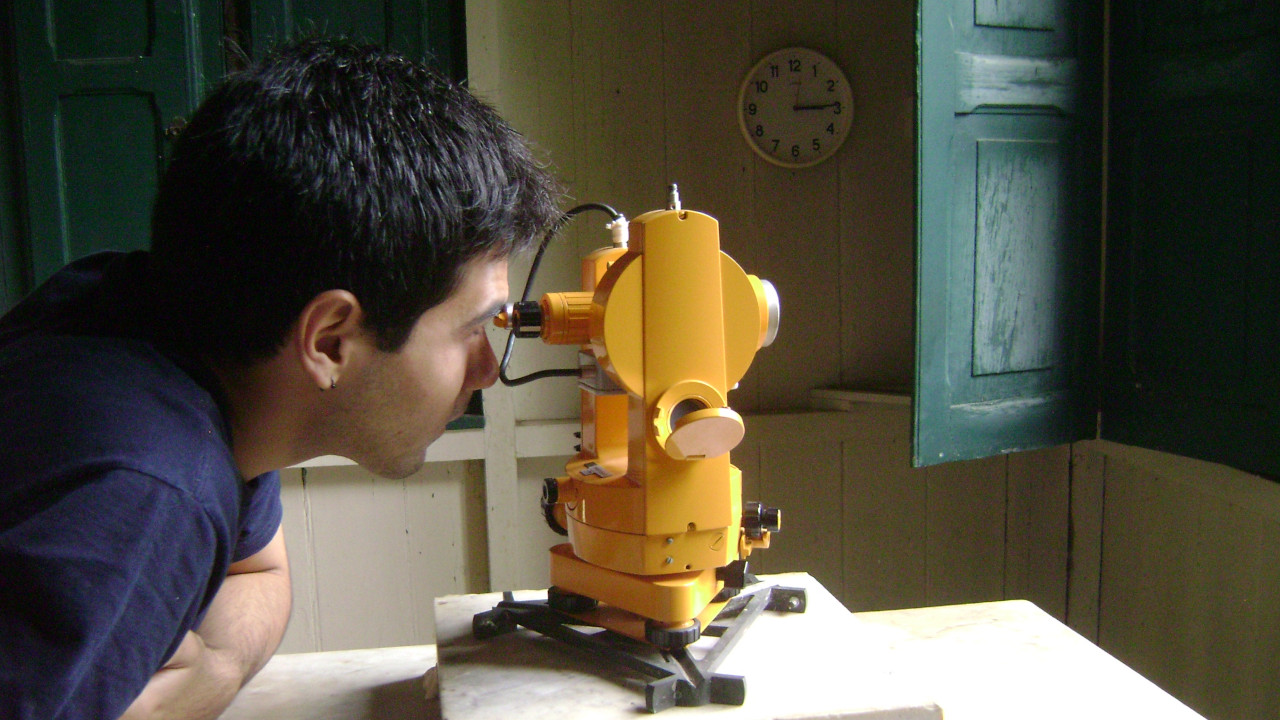
\includegraphics[width=\textwidth]{images/vassouras-geomag-observation-2012.jpg}
  \end{center}
  \caption{
    Realizando medidas da direção do campo geomagnético no observatório de
    Vassouras, Rio de Janeiro. A atividade foi parte de uma disciplina de
    instrumentação geofísica que cursei durante a pós-graduação do Observatório
    Nacional.
  }
\end{figure}
\begin{summarybox}[frametitle=\faInfoCircle{}\quad Resumo da formação acadêmica]
  \begin{datelist}
    2004--2009 & Bacharelado em Geofísica -- Universidade de São Paulo \\
    2008--2009 & \faPlane{} Intercâmbio Internacional -- York University, Canadá \\
    2010--2011 & Mestrado em Geofísica -- Observatório Nacional \\
    2011--2016 & Doutorado em Geofísica -- Observatório Nacional
  \end{datelist}
\end{summarybox}

Este capítulo relata a minha formação acadêmica, do Bacharelado ao Doutorado,
refletindo sobre os fatores que influenciaram minhas linhas de pesquisa e o
rumo que tomei durante minha carreira.

\section{Universidade de São Paulo}
\label{sec_usp}

\begin{subsummarybox}[frametitle=\faGraduationCap{}\quad Bacharelado em Geofísica]
  \begin{fa-ul}
    \faUniversity & Universidade de São Paulo \\
    \faCalendar & Fevereiro 2004 -- Novembro 2009 \\
    \faUser & Orientadora: Naomi Ussami\\
    \faInfoCircle & Trabalho de conclusão: Cálculo do tensor gradiente
    gravimétrico utilizando tesseroides (\DOI{10.6084/m9.figshare.963547})
  \end{fa-ul}
\end{subsummarybox}

Ingressei no curso de Bacharelado em Geofísica da Universidade de São Paulo em
2004.
Já no primeiro semestre, o curso desafio diversos de meus preconceitos sobre os
assuntos abordados.
Uma das experiências mais marcantes foi a disciplina MAC0115 ``Introdução à
Computação para Ciências Exatas e Tecnologia''.
Minha expectativa era aprender sobre funções avançadas de softwares como o
Microsoft Office, talvez aprender sobre algum programa específico para a
geofísica.
Jamais havia imagino que como parte do meu curso de Geofisica eu aprenderia
como criar meus próprios programas, mas foi exatamente isso que aprendemos
nessa disciplina que foi ministrada de maneira excepcional.
Minha carreira com certeza teria tomado um rumo completamente diferente se
minha primeira experiência com a programação não houvesse sido tão positiva.
Aprendi os conceitos básicos da linguagem de programação C e, junto com meu
amigo \href{https://www.linkedin.com/in/balancin/}{Lucas Balancin}, resolvi
todos os exercícios fornecidos para estudo da disciplina.
Porém, não acalcei um nível suficientemente avançado para enxergar aplicações
imediatas da programação nas demais disciplinas do curso.

Busquei aprender mais sobre a programação através da disciplina optativa
AGG0204 ``Computação para Geofísicos''.
Durante a disciplina, desenvolvi aplicações diretas da programação à geofísica
como o cálculo do International Geomagnetic Reference Field (IGRF) a partir dos
coeficientes de harmônicos esféricos.
Essas aplicações me mostraram o enorme poder da programação no aprendizado de
conceitos complexos da geofísica e da matemática.
Ao criar uma implementação computacional de um método, o aluno é levado a
considerar detalhes e a elaborar perguntas que passariam despercebidas ao
estudar somente pela teoria.
Além disso, também é capaz de explorar as possibilidades e os limites de uma
teoria de forma dinâmica e independente.

Nos anos seguintes continuei a estudar programação por mim mesmo nas horas
vagas e a aplicar à geofísica o que estava aprendendo.
Aprendi como programar nas linguagens Java, C++ e Python (por recomendação do
então aluno de mestrado \href{https://www.linkedin.com/in/fspaolo/}{Fernando Paolo}).
Implementei a Transformada Discreta de Fourier\footnote{Disponível em
\url{https://github.com/leouieda/dft-in-c}} para estudar para a disciplina
AGG0330 ``Processamento de Sinais Digitais''.
Utilizei uma implementação do método \textit{Ant Colony Optimization}
\citep{Socha2008}, que fiz por curiosidade própria, para realizar uma inversão
de velocidades de grupo de ondas
Love\footnote{Disponível em \url{https://github.com/leouieda/love-aco-inv}}
como meu projeto para a disciplina AGG0305 ``Teoria de Ondas Sísmicas e
Estrutura da Terra''.
Cursei a disciplina optativa MAC0122 ``Princípios de Desenvolvimento de
Algoritmos'' onde aprendi os conceitos de estruturas de dados e recursividade
que possibilitaram alguns dos avanços que obtive em \citet{Uieda2016}
(seção~\ref{sec_tesseroids}).

O curso também me forneceu treinamento excepcional em quase todos os métodos de
geofísica.
Tivemos experiências de campo e utilizamos uma ampla variedade de equipamentos
geofísicos.
A junção da base teórica sólida com essa experiência prática foi
extremamente motivante para alunos como eu, que estavam indecisos sobre suas
carreiras e qual rumo seguir após a graduação.

Refletindo agora, quase 19 anos após ingressar na USP, percebo o quão sólida
foi a base que adquiri durante a graduação. Utilizo os conceitos que aprendi
nas disciplinas de computação, álgebra linear, física e métodos potenciais
diariamente. Tendo passado por cinco outras instituições no Brasil e no
exterior, reconheço o quão raro é um curso preparar tão bem seus alunos.
Por isso, sou muito grato a todos os meus professores e ao país por me dar
acesso a essa educação de forma gratuita (outra raridade, principalmente no
exterior).

\subsection{Iniciação científica: Paleomagnetismo}

Durante meu segundo ano de graduação, iniciei um projeto de iniciação
científica com o Professor Manoel Souza D'Agrella Filho.
O objetivo do trabalho era obter um paleo-pólo geomagnético para um conjunto
de diques de idade cambriana da região de Maravilhas, Paraíba.
O projeto intitulado ``Paleomagnetismo e mineralogia magnética dos diques
cambrianos de Maravilhas e Prata (PB)'' foi apoiado por uma bolsa da
FAPESP\footnote{Mais informações em
\url{https://bv.fapesp.br/pt/bolsas/73578/paleomagnetismo-e-mineralogia-magnetica-dos-diques-cambrianos-de-maravilhas-e-prata-pb}}
por um ano.
O trabalho incluiu uma expedição para amostrar novos diques na região de
Monteiro, Paraíba, liderado pelo Professor Ricardo I. F. Trindade
(figura~\ref{fig_paleomag}).
Os resultados foram apresentados em um poster no XI Simpósio de Iniciação
Científica do IAG/USP \citep{Uieda2006}.
Essa foi a primeira vez que participei de um projeto de pesquisa e apresentei
um poster.
Sou muito grato ao Manuel e o Ricardo pela oportunidade de aprender mais sobre
o paleomagnetismo e pelas experiências de laboratório e de campo.
Percebi com esse projeto que, embora os resultados e sua interpretação tenham
sido muito interessantes, a rotina de laboratório não era algo que eu
conseguiria manter a longo prazo.
Ao mesmo tempo, estava cada vez mais interessado na computação e modelagem
numérica.
Isso me levou a buscar outra área para continuar minha iniciação científica e
trabalho de conclusão de curso.
Mesmo assim, o paleomagnetismo ainda é um assunto que me interessa muito.
Tanto que, 16 anos depois dessa primeira iniciação científica, estou retornando
ao assunto com uma nova linha de pesquisa em microscopia magnética em
colaboração com o Ricardo (seção~\ref{sec_micromag}).

\begin{figure}[tb]
  \begin{center}
    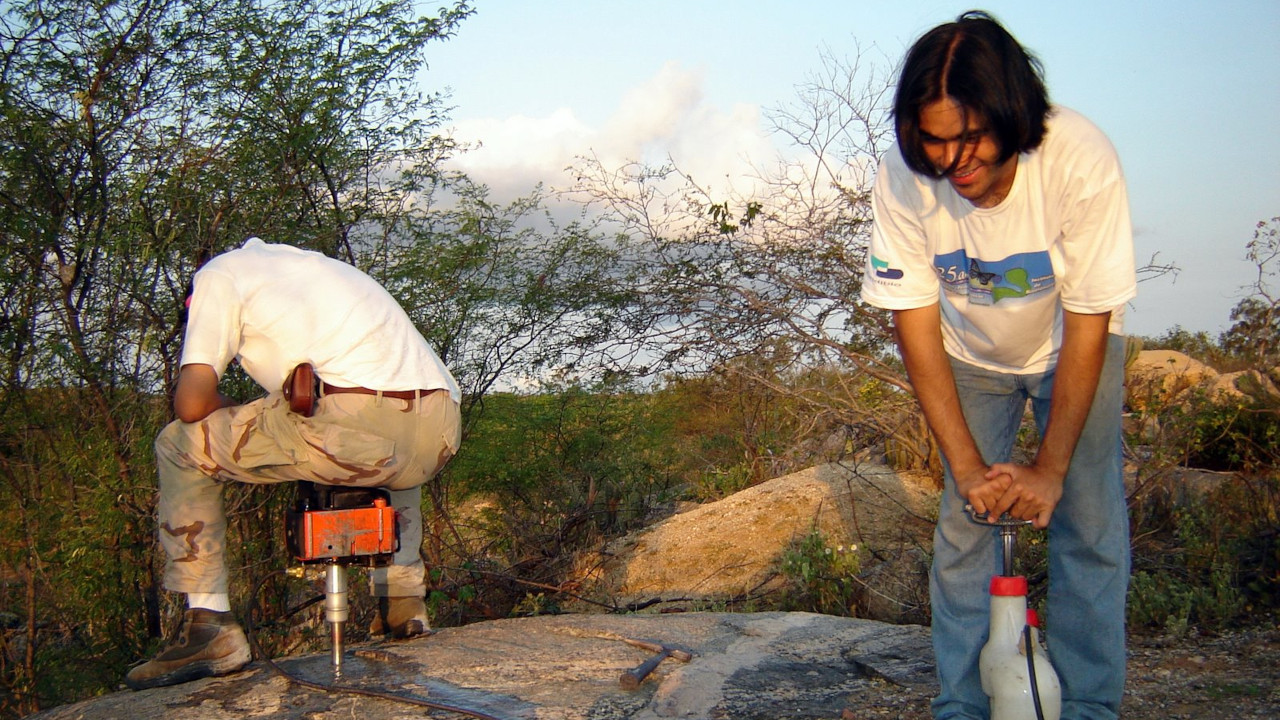
\includegraphics[width=\textwidth]{images/campo-paleomag-2005.jpg}
  \end{center}
  \caption{
    Ricardo (direita) operando a furadeira e eu (esquerda) bombeando água para
    amostrar diques cambrianos durante um trabalho de campo na região de
    Monteiro, Paraíba.
  }
  \label{fig_paleomag}
\end{figure}

\subsection{Iniciação científica: Gravimetria e computação}

No final de 2007, durante meu terceiro ano de graduação, me juntei ao grupo da
Professora Naomi Ussami para trabalho em um projeto que abordava os temas que
mais me interessavam no momento: computação, modelagem numérica e gravimetria.
O projeto intitulado ``Modelagem gravimétrica de corpos tesseroidais'' foi
executado com uma bolsa da
SBGf\footnote{Mais informações em \url{https://sbgf.org.br/programa_ic}}
e em colaboração com a Professora Carla Braitenberg da Università degli studi
di Trieste, Itália.
Nosso objetivo era desenvolver um software que pudesse calcular campos
gravitacionais causado por segmentos de uma esfera (\textit{tesseroides}).
Esse programa seria utilizado para trabalhar com dados da futura missão de
satélite \href{https://www.esa.int/Enabling_Support/Operations/GOCE}{GOCE},
tanto na fase inicial de avaliação de sua sensibilidade a diferentes estruturas
geológicas quanto na fase de processamento e modelagem dos dados obtidos.
Durante as fases iniciais desse projeto, contei com o auxílio da Dra.
Franziska Wild-Pfeiffer, cujo artigo \citep{WildPfeiffer2008} eu estava
tentando reproduzir.
Apresentei meus resultados iniciais no XIII Simpósio de Iniciação Científica do
IAG/USP \citep{Uieda2008}.
No final de 2009, concluí o Bacharelado defendendo o trabalho de conclusão de
curso intitulado ``Cálculo do tensor gradiente gravimétrico utilizando
tesseroides''\footnote{Disponível em \url{https://doi.org/10.6084/m9.figshare.963547}}.

Este trabalho marcou a primeira versão do software Tesseroids
(seção~\ref{sec_tesseroids}), desenvolvido inicialmente na linguagem Python,
e o início de uma linha de pesquisa que abrangeu minha pós-graduação e primeira
coorientação de um aluno de Doutorado (seção~\ref{sec_modelagemdireta}).

\section{York University}
\label{sec_york}

\begin{subsummarybox}[frametitle=\faPlane{}\quad Intercâmbio internacional]
  \begin{fa-ul}
    \faUniversity & York University, Canadá\\
    \faCalendar & Agosto 2008 -- Maio 2009
  \end{fa-ul}
\end{subsummarybox}

Tive o desejo de fazer um intercâmbio no exterior desde o início do curso de
graduação.
Rotineiramente vasculhava as diversas oportunidades divulgadas pela
universidade por uma que oferecesse cursos de Ciências da Terra.
Uma das primeiras que encontrei foi a \href{https://www.yorku.ca/}{York University},
Canadá.
Seu curso de Ciências da Terra oferecia diversas disciplinas que
complementariam minha formação na USP, principalmente na área de geodésia.
Me inscrevi no processo seletivo interno da USP para concorrer a uma única vaga
que estava sendo ofertada para alunos de todos os cursos da universidade.
Felizmente fui selecionado e me mudei para Toronto, Canadá, em Agosto de 2008.

Tive uma surpresa ao chegar na York e me apresentar na secretaria de graduação:
o curso de Ciências da Terra havia sido descontinuado no ano anterior por causa
do baixo número de alunos inscritos.
Aparentemente, a página online do curso não havia sido atualizada e por isso
eu baseei meu plano de estudos para o ano em curso inexistente.
Por sorte, a maioria das disciplinas que eu havia escolhido cursar ainda
seriam oferecidas como parte de outros cursos.
Os meus estudos acabaram não sendo tão afetados mas minha experiência não foi
como eu esperava por não ter uma turma de alunos de geociências cursando as
mesmas disciplinas, como era o caso na USP.

Durante minha estadia na York, aprendi sobre sistemas geográficos de
coordenadas, posicionamento, ajustes de redes geodésicas, geodésia física e
levantamentos gravimétricos de alta precisão.
Um destaque dessa experiência foram as aulas do Professor
\href{https://www.yorku.ca/spiros/spiros.html}{Spiros Pagiatakis}.
Suas aulas de geodésia e matemática forneceram a clareza que me faltava nos
conceitos de anomalias da gravidade e a solução prática de problemas inversos
em geofísica.
Observando outros alunos presentes na disciplina, considero que somente pude
aproveitar plenamente essas aulas graças à base sólida que tinha obtido em
outras disciplinas da USP.

Meu tempo em Toronto foi excelente para meu crescimento pessoal, cultural e
acadêmico.
Fiz amizade com pessoas de todos os cantos do planeta (Europeus, Asiáticos,
Canadenses) com os quais mantenho contato até hoje.
O conhecimento que adquiri nas disciplinas me possibilitaram começar a
trabalhar diretamente no meu projeto de Mestrado pois já possuía grande parte
da base teórica e experiência prática computacional necessária.
Por isso, fui capaz de desenvolver um método novo em pouco tempo.

\section{Observatório Nacional}
\label{sec_on}

\begin{subsummarybox}[frametitle=\faGraduationCap{}\quad Mestrado em Geofísica]
  \begin{fa-ul}
    \faUniversity & Observatório Nacional \\
    \faCalendar & Fevereiro de 2010 -- Outubro de 2011 \\
    \faUser & Orientadora:  Valéria C. F. Barbosa\\
    \faInfoCircle & Dissertação: Robust 3D gravity gradient inversion by
    planting anomalous densities (\DOI{10.6084/m9.figshare.16882300})
  \end{fa-ul}
\end{subsummarybox}
\begin{subsummarybox}[frametitle=\faGraduationCap{}\quad Doutorado em Geofísica]
  \begin{fa-ul}
    \faUniversity & Observatório Nacional \\
    \faCalendar & Novembro de 2011 -- Abril de 2016 \\
    \faUser & Orientadora:  Valéria C. F. Barbosa\\
    \faInfoCircle & Tese Modelagem direta e inversão de campos gravitacionais em
    coordenadas esféricas (\DOI{10.6084/m9.figshare.16883689}) \\
    \faTrophy & Ganhador do Prêmio SBGf de Melhor Tese de Doutorado (2015--2017)\footnotemark
  \end{fa-ul}
\end{subsummarybox}
\footnotetext{Mais informações em \url{https://sbgf.org.br/premiacoes}}

Minha ida para o Canadá durante a graduação fez com que eu atrasasse minha
formatura em um ano.
Ao retornar, comecei a explorar as opções do que fazer após terminar a
graduação.
Após conversar com meus amigos que já estavam formados e trabalhando em
empresas voltadas à indústria do petróleo no Rio de Janeiro, cheguei à
conclusão de que ainda gostaria de continuar meus estudos e expandir minhas
atividades de pesquisa.
Minha experiência no Canadá me mostrou o quão beneficial é a exposição a uma
diversidade de formas de pensamento que se obtém em diferentes instituições.
Por isso, após cinco anos na USP, decidi que estava na hora de buscar uma
pós-graduação em outra instituição no Brasil.

O Observatório Nacional (ON) já havia despertado meu interesse após uma visita
que fizemos à instituição em 2007 durante uma viagem de nossa turma de
graduação para participar do Congresso Internacional da Sociedade Brasileira de
Geofísica.
Além disso, meu amigo e colega de turma
\href{https://www.pinga-lab.org/people/oliveira-jr.html}{Vanderlei C. Oliveira Jr.}
já havia se formado e estava cursando o Mestrado em Geofísica do Observatório
Nacional (ON) sob supervisão da Professora
\href{https://www.pinga-lab.org/people/barbosa.html}{Valéria C. F. Barbosa}.
Após uma visita ao Rio de Janeiro em 2009, o Vanderlei me convenceu (sem muito
esforço) a me inscrever no Mestrado do ON ao terminar a graduação na USP.
Ele também convenceu a Valéria a me orientar, o que considero ser um dos
maiores favores que um amigo jamais me fez.
Sou eternamente grato ao Vanderlei pela recomendação e à Valéria por aceitar me
orientar.

O ambiente da pós-graduação do ON era extremamente produtivo e estimulante.
As salas misturavam alunos dos diversos grupos de pesquisa da astronomia e
geofísica, facilitando o intercâmbio de ideias entre os alunos.
Por exemplo, aprendi muito sobre o processamento de dados sísmicos e de GPR
ajudando meu amigo e colega de sala
\href{https://www.linkedin.com/in/saulo-siqueira-martins-78770878/}{Saulo Siqueira Martins}
(atualmente Professor de Geofísica da Universidade Federal do Pará)
a utilizar o software \href{https://www.reproducibility.org/}{Madagascar}.
Essa conhecimento foi extremamente útil nas minhas atividades de ensino na
\UERJ{} (capítulo~\ref{cap_ensino}).

A pós-graduação também me forneceu diversas oportunidades de frequentar
congressos internacionais com financiamento da CAPES e de projetos da Valéria.
Essas participações me ajudaram a estabelecer contatos e criar uma rede de
apoio e colaboração internacional.
Por exemplo, os contatos que fiz no congresso
\href{https://conference.scipy.org/scipy2014/}{Scipy} de 2013 e 2014 levaram a
minha participação na diretoria do
\href{https://softwareunderground.org/}{Software Underground}, a organização
de seções em congressos e colaborações com os desenvolvedores do software
\href{https://simpeg.xyz/}{SimPEG}.
O incentivo e a liberdade de escolher meus temas de pesquisa dados pela Valéria
sempre me motivaram a dar o melhor de mim.
Não exagero quando afirmo que conhecer a Valéria foi o acontecimento mais
influente na minha carreira.

Durante a pós-graduação, continuei a perseguir meu interesse na programação,
no software libre e na ciência aberta.
Aprendi como usar o sistema de controle de versão
\href{https://git-scm.com/}{git} e a plataforma
\href{https://github.com}{GitHub} e como criar páginas da internet com HTML e
CSS.
Continuei o desenvolvimento do software \href{https://tesseroids.leouieda.com/}{Tesseroids}
e criei o projeto \href{https://www.fatiando.org}{Fatiando a Terra}
(seção~\ref{sec_fatiando}) junto com alguns colegas da graduação, includindo o
Vanderlei.
O investimento inicial que fiz na qualidade do código do Fatiando me
permitiu terminar meu projeto de Mestrado em apenas 18 meses,
concluir minha tese de Doutorado enquanto já trabalhava como Professor
Assistente na UERJ (seção~\ref{sec_uerj} e elaborar aulas interativas sobre
geofísica para meus alunos de geologia.

Em meados de 2013, eu, o Vanderlei e a Valéria iniciamos o grupo de
\href{https://www.pinga-lab.org/}{\textbf{P}roblemas \textbf{In}versos em \textbf{G}eofísic\textbf{a}}
(PINGA).
A conta do grupo no GitHub\footnote{Disponível em \url{https://github.com/pinga-lab}}
agrega os repositórios com o código fonte para reproduzir as publicações do
grupo.
O grupo também conta com uma página na internet\footnote{Página do grupo PINGA: \url{https://www.pinga-lab.org}},
feita em grande parte por mim\footnote{Sou o maior contribuidor em termos de
linhas de código geradas:
\url{https://github.com/pinga-lab/website/graphs/contributors}.},
onde divulgamos as teses, artigos, projetos e integrantes do grupo.

\subsection{Mestrado}

Meu projeto de mestrado era adaptar o método desenvolvido
pela Valéria e seu ex-aluno
\href{https://www.researchgate.net/profile/Fernando-Dias-8}{Fernando Silva Dias}
\citep{SilvaDias2009} para inverter dados de gradiente da gravidade.
Na época, esse tipo de dado estava começando a ser utilizado na área de
recursos minerais mas ainda havia uma falta de métodos de inversão 3D para sua
interpretação.
O projeto estava atrelado ao projeto de Doutorado do aluno
\href{https://www.linkedin.com/in/dionisio-uendro-carlos-093671225/}{Dionisio Uendro Carlos},
que iria utilizar o método desenvolvido por mim para interpretar dados
fornecidos pela empresa \href{https://vale.com/}{Vale}.

A abordagem que eu preferia (e prefiro até hoje) para compreender um assunto
novo é fazer por mim mesmo a implementação computacional de todos os conceitos
básicos e reproduzir resultados existentes.
Logo, comecei meu Mestrado implementando novamente o método de \citet{Nagy2000}
e toda a base para gerar dados sintéticos, resolver problemas inversos lineares
3D e visualizar em 3D os resultados da inversão.
Esse código formou a base do projeto
\href{https://www.fatiando.org}{Fatiando a Terra} e ainda sobrevive em partes
de sua encarnação atual (seção~\ref{sec_fatiando}).
Minha vontade era encontrar uma abordagem nova, ao invés de simplesmente seguir
o que já havia sido feito em \citet{SilvaDias2009}.
Sendo uma orientadora consciente, a Valéria corretamente me deu somente até o
final de meu primeiro ano para explorar diferentes opções.
Caso não fosse capaz de desenvolver um método novo, combinamos que eu faria o
projeto inicialmente proposto.
Tendo esse prazo em mente, trabalhei incessantemente durante o ano de 2010 para
desenvolver uma abordagem nova de inversão.

Minha grande descoberta veio quando me deparei com o trabalho de
\citet{Rene1986}.
Este trabalho relativamente desconhecido propôs um método de inversão 2D de
dados de gravidade pouco convencional.
Seu método adiciona elementos iterativamente à solução em torno de ``sementes''
e evita a solução de sistemas lineares, um dos grandes empecilhos
computacionais para a inversão 3D.
Porém, esse trabalho não explorou completamente as vantagens que o conceito de
construir a solução iterativamente possibilitava.
Baseado nas ideias de \citet{Rene1986}, criei um método capaz inverter de
maneira conjunta dados de gravimetria tradicional e gradiometria gravimétrica
em três dimensões.
Adicionei diversas inovações ao método para torná-lo viável a modelos da ordem
de milhões de elementos e melhor controlar a forma do modelo final.
Essas inovações são resultado direto do meu interesse pela computação, podendo
ser rastreadas às disciplinas que cursei ainda na graduação.
O resultado foi publicado em meu primeiro artigo \citep{Uieda2012}, que formou minha
dissertação e foi apresentado nos congressos internacionais da
Society of Exploration Geophysicists,
European Association of Geoscientists and Engineers,
e Sociedade Brasileira de Geofísica
(seção~\ref{sec_planting}).
Esse artigo também foi meu primeiro experimento em ciência aberta.
Todo o código para produzir os resultados e figuras do artigo foi publicado
em um repositório do GitHub\footnote{Disponível em
\url{https://github.com/pinga-lab/paper-planting-densities}} e o material
suplementar foi publicado no
\href{https://figshare.com/}{figshare}\footnote{Disponíveis em
\url{https://doi.org/10.6084/m9.figshare.91574} e
\url{https://doi.org/10.6084/m9.figshare.91469}}.

Terminei meu mestrado em Outubro de 2011 (quatro meses adiantado) e ingressei
no Doutorado em Geofísica do Observatório Nacional, ainda sob supervisão da
Valéria, logo em seguida.

\subsection{Viagem para Trieste}

Em 2011, ainda no Mestrado, fui convidado pela Professora Carla Braitenberg
para passar um mês na Università degli studi di Trieste, Itália, para continuar
o desenvolvimento do software Tesseroids.
Passei Fevereiro de 2011 trabalhando com ela em uma nova versão do software
escrito em linguagem C.
Na época, produzir um software numérico em Python que pudesse alcançar a
performance de programas escritos em C não era uma tarefa fácil.
Por isso, decidimos que a melhor alternativa seria reescrever o software em C.
Essa nova versão mais eficiente do programa seria necessária para o
processamento de dados do satélite GOCE que o grupo de Trieste almejava fazer.
Durante minha estadia em Trieste, reescrevi o software na linguagem C, criei
uma página para a documentação\footnote{Disponível em \url{https://tesseroids.leouieda.com}}
e desenvolvi um algoritmo de discretização adaptativa para combater o problema
de estabilidade numérica do método\footnote{O \textit{commit} 0af974f
introduziu a discretização adaptativa de tesseroides em 11 de Fevereiro de
2011:
\url{https://github.com/leouieda/tesseroids/commit/0af974f26a15f98f1072ccc6c4ebf29588863f51}}.

\subsection{Doutorado}

Meu projeto de Doutorado era desenvolver métodos para inversão de dados de
gravidade 3D em uma aproximação esférica da Terra, combinando assim os temas
do meu trabalho de conclusão de curso de graduação e dissertação de Mestrado.
A aproximação esférica é necessária para a modelagem em escala continental e
global.
Também decidimos que o desenvolvimento dos softwares Tesseroids e Fatiando a
Terra seriam parte dos objetivos principais da tese.
Esses programas seriam os principais ``produtos'' gerados pelo meu Doutorado
para a comunidade científica.

Os dois primeiros anos do meu Doutorado foram dedicados ao desenvolvimento dos
programas e à colaborações com outros membros do recém-formado
\href{https://www.pinga-lab.org}{PINGA}.
Participei da concepção, execução e escrita dos trabalhos
\citet{OliveiraJr2013}, \citet{Melo2013}, \citet{Carlos2014},
\citet{OliveiraJr2015} e \citet{Carlos2016}.
Expandi a gama de funções disponíveis no Fatiando a Terra\footnote{Ver lista
de mudanças nas versões v0.1 e v0.2 em \url{https://legacy.fatiando.org/changelog.html}}
e apresentei meus trabalhos em diversos congressos internacionais.

No final de 2013, me inscrevi e fui aprovado no concurso público para a vaga de
Professor Assistente no Departamento de Geologia Aplica da \UERJ
(seção~\ref{sec_uerj}).
Entre 2014 e 2016, exerci minhas tarefas de docente da UERJ enquanto terminava
os trabalhos \citet{Uieda2016} e \citet{Uieda2017}.
Esses dois anos foram muito desafiadores, principalmente no período de
adaptação ao meu novo cargo de Professor.
Graças ao investimos que havia feito no Fatiando a Terra nos quatro anos
anteriores, fui capaz de desenvolver, aplicar e publicar o método descrito em
\citet{Uieda2017} durante o pouco tempo vago que tive em 2015 e
2016\footnote{O primeiro \textit{commit} do repositório do GitHub do artigo é
de Março de 2015: \url{https://github.com/pinga-lab/paper-moho-inversion-tesseroids/commit/edd0e33a200bd1946be0020a38d1d362d93f2c36}}.
Em Abril de 2016, defendi minha tese de Doutorado intitulada ``Modelagem direta
e inversão de campos gravitacionais em coordenadas esféricas'', composta pelos
trabalhos \citet{Uieda2013}, \citet{Uieda2016} e \citet{Uieda2017}.
Fui ganhador do Prêmio SBGf de Melhor Tese de Doutorado
(2015--2017)\footnote{Mais informações em \url{https://sbgf.org.br/premiacoes}}
e esses três artigos estão entre meus trabalhos com maior número de
citações\footnote{Segundo o Google Scholar em 27/12/2022:
\url{https://scholar.google.com/citations?user=qfmPrUEAAAAJ&hl=en}}.


\section{Formação complementar em pedagogia}

Minha formação no Bacharelado, Mestrado e Doutorado me prepararam bem para uma
carreira de pesquisa.
Porém, senti que ainda havia lacunas no meu treinamento, principalmente na área
de ensino.
Busquei preencher essas lacunas através dos cursos complementares em técnicas
práticas de ensino e teoria pedagógica descritos abaixo.

\subsection{Software Carpentry}
\label{sec_swcarpentry}

\begin{subsummarybox}[frametitle=\faGraduationCap{}\quad The Carpentries Instructor Training]
  \begin{fa-ul}
    \faUniversity & \href{https://carpentries.org/}{The Carpentries} \\
    \faCalendar & 9--10 de Julho de 2018\\
    \faInfoCircle & Habilitação para organizar e ministrar os cursos
    \textit{Software Carpentry}, \textit{Data Carpentry} e
    \textit{Library Carpentry}, incluindo treinamento em pedagogia e práticas
    de ensino de programação e ciência de dados
  \end{fa-ul}
\end{subsummarybox}

Me deparei com o \href{https://software-carpentry.org/}{Software Carpentry}
em 2008 durante meu intercâmbio na York University.
Na época, a organização consistia de uma página na internet com informações
para treinamento de cientistas em técnicas de engenharia de
software\footnote{Infelizmente, a versão do material de 2008 só está disponível
no repositório \url{https://github.com/swcarpentry/v3}}.
Esse material abriu meus olhos para o mundo da engenharia de software que ia
muito além das disciplinas de programação que cursei na USP durante minha
graduação.
Passei grande parte do meu tempo livre durante os meses de inverno no Canadá
imerso no Software Carpentry, aprendendo sobre o sistema de controle de versão
\href{https://subversion.apache.org/}{subversion} (precursor do
\href{https://git-scm.com/}{git}), testes unitários, programação defensiva,
automatização com o \href{https://www.gnu.org/software/make/}{GNU Make},
expressões regulares, programação em
\href{https://www.gnu.org/software/bash/}{bash}, entre outros.
Busquei aplicar esses conceitos novos imediatamente, tanto para as tarefas das
disciplinas que estava cursando quanto para meu trabalho de conclusão de curso
e o programa Tesseroids.
Utilizo todas a lições que aprendi com o Software Carpentry diariamente na
minha pesquisa, ensino e até mesmo para escrever esse memorial (armazenado em
um repositório privado no GitHub e utiliza o Make para compilação do código
\LaTeX{}).

Atualmente, o Software Carpentry é parte da organização sem fins lucrativos
\href{https://carpentries.org/}{The Carpentries}, que promove
internacionalmente cursos de curta duração em engenharia de software para
cientistas.
Os cursos são ministrados, e frequentemente organizados, voluntariamente por
instrutores credenciados.
Em 2018, realizei o curso de habilitação de instrutores do The Carpentries e me
tornei um instrutor
credenciado\footnote{Mais informações em \url{https://carpentries.org/instructors/\#leouieda}}.
O curso cobre técnicas para ensino de programação baseadas em evidências da
literatura pedagógica \citep[resumidas em][]{Brown2018}.
A habilitação me permite organizar e ministrar cursos oficiais do The
Carpentries.

Utilizo as técnicas aprendidas tanto em minhas aulas de programação em Python
como nas aulas de geofísica que possuem uma componente computacional
(capítulo~\ref{cap_ensino}), que são a grande maioria as aulas que dou
atualmente.
A experiência que tive com o uso eficaz de tecnologias para ensino virtual que
foram utilizadas nas etapas finais do curso (Zoom, Google Docs, etc.) foram
extremamente valiosas durante a transição para o ensino online causada pela
pandemia de COVID em 2020 e 2021.


\subsection{Pedagogia no ensino superior}
\label{sec_pgcap}

\begin{subsummarybox}[frametitle=\faGraduationCap{}\quad Postgraduate Certificate in Academic Practice]
  \begin{fa-ul}
    \faUniversity & Universidade de Liverpool \\
    \faCalendar & Novembro de 2020 -- Maio de 2022 \\
    \faInfoCircle & Curso de pós-graduação em pedagogia no ensino superior que
    me confere o título de \textit{Fellow of the Higher Education
    Academy} (número de referência PR242069)
  \end{fa-ul}
\end{subsummarybox}

Durante meu segundo em Liverpool, realizei o curso de pós-graduação
Postgraduate Certificate in Academic Practice (PGCAP) oferecido pela Faculty
of Humanities and Social Sciences da universidade.
A conclusão do PGCAP em 2022 me conferiu o título de \textit{Fellow of the
Higher Education Academy}\footnote{Mais informações em
\url{https://www.advance-he.ac.uk/fellowship/fellowship}},
que é necessário para progressão na carreira acadêmica nas instituições da
Inglaterra.
O curso foi divido em duas partes:
a primeira composta de aulas sobre teórica pedagógica aplicada ao ensino
superior e a segunda composta de um projeto de pesquisa ou revisão em
pedagogia.

Meu projeto para a segunda parte do curso foi uma revisão bibliográfica sobre
a técnica de observação por pares aplicada ao ensino superior
\citep{Cosh1998,Fletcher2018,OKeeffe2021}.
Observação por pares se refere a diversas técnicas que envolvem professores
assistirem e revisarem aulas de outros professores.
Resolvi abordar esse tema após realizar uma sessão de observação por pares
durante a primeira parte do curso.
De todas as atividades que fizemos no PGCAP, essa foi a que mais me beneficiou
e me pareceu ter o maior potencial para difundir boas práticas pedagógicas
entre os professores.
Minha revisão bibliográfica e demais reflexões e notas do curso estão
disponíveis em \url{https://www.leouieda.com/pgcap}.


%==============================================================================
\chapter{Atuação Profissional}
\label{cap_atuacao}

\begin{figure}[h]
  \HeroFigPad
  \begin{center}
    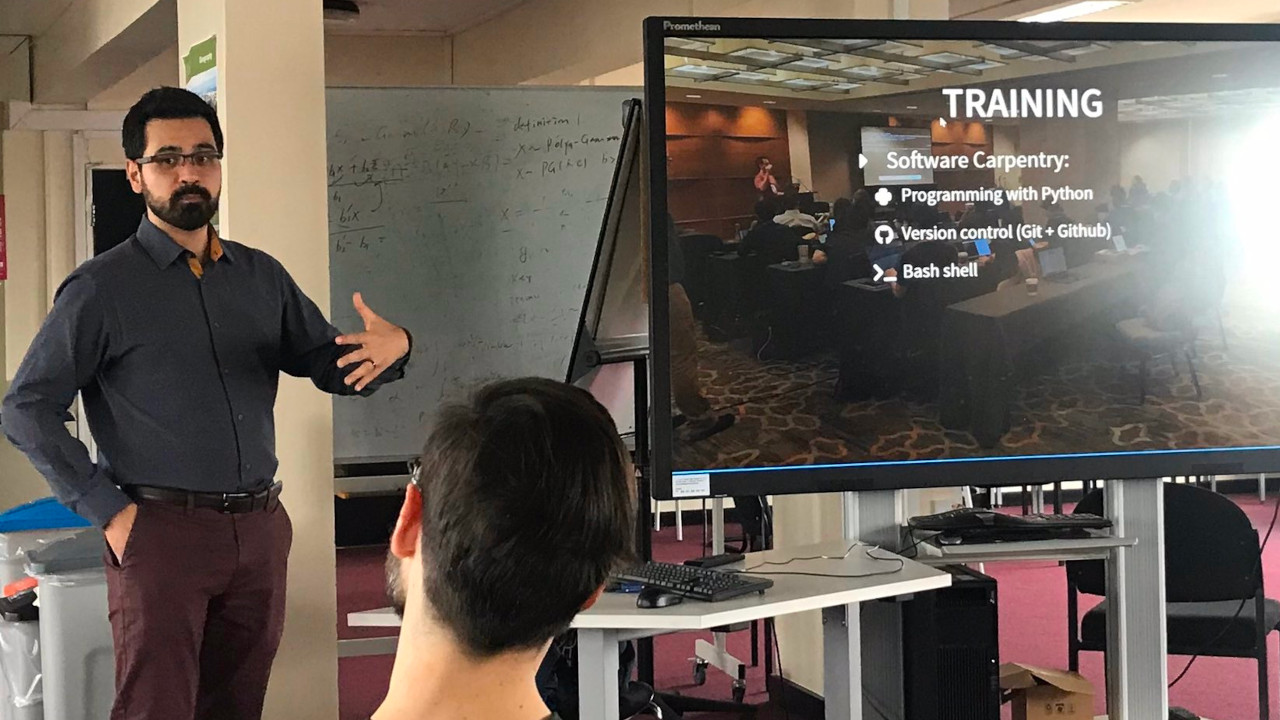
\includegraphics[width=\textwidth]{images/liverpool-gdsl.jpg}
  \end{center}
  \caption{
    Foto de uma apresentação que fiz para o \textit{Geographic Data Science
    Lab} da Universidade de Liverpool em Março de 2020. O propósito da palestra
    foi me apresentar para o grupo pouco após minha chegada em Liverpool e
    tentar estabelecer temas para colaborações futuras.
  }
\end{figure}
\begin{summarybox}[frametitle=\faInfoCircle{}\quad Resumo da atuação profissional]
  \renewcommand{\thempfootnote}{$\dagger$}
  \begin{datelist}
    2014--2018 & Professor Assistente -- \UERJ \\
    2017--2019 & Pesquisador Visitante -- \UHM, E.U.A. \\
    2019--2022 & Topic Editor\footnote{Posição voluntária} -- Journal of Open Source Software (voluntário) \\
    2019--2022 & Advisory Council Member\mpfootnotemark[\value{mpfootnote}] -- EarthArXiv \\
    2019--atual & Lecturer (\textit{Professor Doutor}) -- University of Liverpool, Reino Unido \\
    2022--atual & Board Member\mpfootnotemark[\value{mpfootnote}] -- Software Underground \\
    2022--atual & Advisory Committee Member\mpfootnotemark[\value{mpfootnote}] -- pyOpenSci
  \end{datelist}
\end{summarybox}

Este capítulo relata minha atuação profissional, tanto como funcionário em
instituições de ensino superior, quanto como voluntário em posições de
liderança em organizações sem fins lucrativos que servem a comunidade
científica.
Os relatos abaixo se referem somente à atividades institucionais e experiências
pessoas.
Minhas linhas de pesquisa (incluindo a orientação de alunos) e atividades de
ensino e extensão serão discutidas nos capítulos~\ref{cap_pesquisa},
\ref{cap_ensino} e \ref{cap_extensao}, respectivamente.


\section{\UERJ}
\label{sec_uerj}

\begin{subsummarybox}[frametitle=\faUniversity{}\quad Vínculo institucional]
  \begin{fa-ul}
    \faUser & Professor Assistente \\
    \faMapMarker & Departamento de Geologia Aplicada -- Faculdade de Geologia \\
    \faCalendar & Fevereiro 2014 -- Janeiro 2018\footnotemark{} \\
    \faTrophy & Paraninfo da turma de formandos da Geologia (ano de ingresso 2012)
  \end{fa-ul}
\end{subsummarybox}
\footnotetext{Afastado entre Fevereiro de 2017 e Janeiro de 2018 para trabalhar na \UHM{}}
\begin{subsummarybox}[frametitle=\faList{}\quad Atividades institucionais]
  \begin{datelist}
    2014--2017 & Coordenador: Laboratório de Geofísica de Exploração (LAGEX) \\
    2014--2017 & Coordenador: Projeto Qualitec para contratação de um bolsista de nível superior para atuar no LAGEX \\
    2015--2017 & \textit{Faculty Advisor}: Capítulo Estudantil da Society of Exploration Geophysicists (\textit{UERJ Geophysical Society}) \\
    2015 & Representante docente titular da sub-comissão eleitoral da Faculdade de Geologia
  \end{datelist}
\end{subsummarybox}

No final de 2013, durante meu segundo ano do Doutorado, surgiu a oportunidade
de prestar o concurso público para cargo de Professor Assistente na \UERJ{}
(UERJ).
Somente era necessário o título de Mestre e o concurso era para a área de
Geofísica.
Por recomendação da minha orientadora Valéria C. F. Barbosa, decidi prestar o
concurso pois seria excelente oportunidade iniciar uma carreira acadêmica antes
mesmo de terminar meu Doutorado.
Felizmente, fui aprovado em primeiro lugar no concurso e tomei posse do cargo
de Professor Assistente na UERJ em Fevereiro de 2014.
De início, assumi a posição de coordenador do Laboratório de Geofísica de
Exploração (LAGEX) e a responsável por duas novas disciplinas de geofísica
do Bacharelado em Geologia e outras disciplinas do Bacharelado em Oceanografia
(seção~\ref{sec_ensino_uerj}).

Na coordenação do LAGEX, liderei nossa aplicação para uma chamada de projetos
interna da UERJ (QUALITEC) que forneceria financiamento para a
contratação de um bolsista de nível superior por quatro anos.
Nossa aplicação foi bem sucedida e no final de 2014 nomeei o
\href{https://www.linkedin.com/in/victorxalmeida/}{Victor Thadeu Xavier de Almeida}
para assumir a bolsa.
O Victor era responsável pela manutenção dos computadores GNU/Linux do LAGEX,
por auxiliar no ensino de disciplinas de graduação que utilizavam o
laboratório e também por contribuir com o desenvolvimento do Fatiando a Terra.
Ter o Victor no LAGEX durante minha estadia foi excelente e ele elevou minhas
contribuições de ensino, pesquisa e desenvolvimento do Fatiando.

Ainda em 2014, trabalhei com os alunos
\href{https://www.linkedin.com/in/caroline-adolphsson-61723137/}{Caroline Adolphsson Nascimento}
e \href{https://www.linkedin.com/in/gustavo-pereira-780839111/}{Gustavo do Couto Ramos Pereira}
para fundar um capítulo estudantil da
\href{https://seg.org}{Society of Exploration Geophysicists} (SEG) na UERJ.
Os capítulos da SEG proporcionam diversas oportunidades de desenvolvimento
profissional para os alunos através do financiamento de sua participação no
congresso anual nos E.U.A., campeonatos regionais e ciclos de palestras
internacionais.
O capítulo, denominado ``State University of Rio De Janeiro Geophysical
Society'' foi fundado oficialmente em Janeiro de 2015 e ainda encontra-se em
operação\footnote{Segundo \url{https://seg.org/Education/Student/Student-Chapters/Student-Chapter-Details/student-chapter-listing-details/scID/000000440245} (acessado em 03/01/2023)}.

Após terminar meu doutorado em 2016, comecei a cogitar pedir um afastamento de
um ano para fazer um pós-doutorado fora do país.
Isso foi motivado em partes pelo meu cansaço após dois intensos anos
trabalhando em período integral enquanto terminava o Doutorado, mas também em
parte por que minha parceira (e atual esposa)
\href{https://www.acarolcolombo.com/}{Ana Caroline Colombo} iria passar um ano
na \href{https://www.stonybrook.edu/}{Stony Brook University} nos Estados
Unidos como parte de seu doutorado.
A oportunidade de continuarmos no mesmo país surgiu na forma do cargo de
Pesquisador Visitante na
\href{https://www.hawaii.edu/}{\UHM{}} para trabalhar com o
\href{https://www.generic-mapping-tools.org/}{Generic Mapping Tools} (GMT),
um dos projetos de software livre de maior impacto na geofísica.
Essa oportunidade era muito boa para ser passada e então pedi meu afastamento
da UERJ por um ano a partir de Fevereiro de 2017.

Uma escolha muito mais desafiadora se apresentou em Janeiro de 2018 quando meu
afastamento chegaria ao fim.
Meu envolvimento no GMT estava sendo proveitoso e havia financiamento para me
manter no cargo por mais um ano e meio, com a possibilidade de conseguirmos
mais recursos no futuro.
Ao mesmo tempo, as condições financeiras e sociais no Brasil continuaram a
piorar, principalmente no Rio de Janeiro.
A UERJ se encontrava em grave situação financeira, causando o atraso no
pagamento dos servidores.
A escolha entre a certeza do meu cargo na UERJ e a incerteza de uma posição
temporária nos Estados Unidos não foi fácil.
Por fim, decidi que a melhor escolha para mim e para minha família naquela fase
da nossa vida seria tentar a sorte no exterior e pedir exoneração do cargo da
UERJ.

Minha experiência na UERJ foi positiva e muito educativa.
Avancei minhas linhas de pesquisa e fiz amizades com outros professores e
servidores da Faculdade de Geologia.
Também foi na UERJ que eu tive confirmação de que é da interação com os alunos,
tanto no papel de professor quanto de mentor, que tiro a maior satisfação
profissional.
Meus esforços foram reconhecidos pelos alunos pois tive a honra de ser
escolhido como paraninfo da turma de formandos da Geologia em 2016 (ano de
ingresso 2012), que foi a primeira turma a qual dei aulas de geofísica.


\section{\UHM}

\begin{subsummarybox}[frametitle=\faUniversity{}\quad Vínculo institucional]
  \begin{fa-ul}
    \faUser & Pesquisador Visitante \\
    \faMapMarker & Department of Earth Sciences -- School of Ocean and Earth Science and Technology\\
    \faCalendar & Fevereiro 2017 -- Agosto 2019
  \end{fa-ul}
\end{subsummarybox}

Comecei a contemplar a possibilidade de fazer um pós-doutorado no exterior
após defender minha tese de doutorado em meados de 2016.
Na busca por oportunidades de financiamento, me inscrevi em todas as listas de
email e classificados que pude encontrar\footnote{Até escrevi um artigo no
meu blog com uma lista desses recursos:
\url{https://www.leouieda.com/blog/job-sites.html}}.
Foi assim que me deparei com um email do Professor
\href{https://www.soest.hawaii.edu/pwessel/}{Paul Wessel} divulgando uma
posição para desenvolver uma ponte entre o software
\href{https://www.generic-mapping-tools.org/}{Generic Mapping Tools} (GMT)
e a linguagem de programação Python.
Tanto o Paul quanto o GMT são mundialmente famosos e o meu perfil se encaixava
perfeitamente na descrição das qualificações necessárias para a vaga.
Após uma entrevista por vídeo conferência com o Paul
e outros desenvolvedores do GMT, fui informado de que havia sido selecionado
para a vaga.
Em Fevereiro de 2017 me mudei do Rio de Janeiro para Honolulu, E.U.A., para
começar essa nova etapa.

Conhecer e trabalhar com o Paul foi o destaque da minha estadia na
\UHM{} (UH).
Aprendi muito com ele, não somente sobre desenvolvimento de software mas sobre
como o sistema acadêmico americano funciona, como escrever projetos para
agências de fomento, como ser um líder que eleva as pessoas ao meu redor e como
ser humilde e reconhecer todos os fatores externos que possibilitam nosso
sucesso.
O jeito descontraído, humoroso e energético do Paul é contagiante.
Sua paixão e brilhantes contribuições para a ciência são fruto de uma vida
fazendo exatamente o que mais gosta.

Minha experiência na UH foi diversa, includindo participações em congressos e
até uma experiência de três dias no navio científico
\href{https://www.soest.hawaii.edu/soestwp/tech/watercraft/kilo-moana/}{R/V Kilo Moana}.
Criei uma rede de colaborares nos E.U.A. através do Paul, principalmente com
o grupo do Professor \href{https://topex.ucsd.edu/sandwell/}{David Sandwell}
do Scripps Institution of Oceanography.
Esse grupo desenvolve o software \href{https://github.com/gmtsar}{GMTSAR} para
processamento de dados de Synthetic Aperture Radar (SAR) e a geração de
interferogramas com a técnica InSAR.
Íamos ao Scripps anualmente para trabalhar com o grupo no software e ajudar a
ministrar o curso de GMT e GMTSAR que era promovido pela organização
\href{https://www.unavco.org/}{UNAVCO} (seção~\ref{sec_workshops}).
Minhas contribuições para o GMT serão discutidas mais adiante na
seção~\ref{sec_gmt}.

O tempo que passei em Honolulu foi inesquecível.
Porém, quando comecei a avaliar as opções para permanecer a longo prazo na UH
ou outra instituição do país, percebi que a carreira acadêmica nos E.U.A. era
excessivamente estressante e incerta.
Como eu e minha esposa sentimos que ainda não estávamos prontos para retornar
ao Brasil, retomei minha busca por oportunidades de emprego no exterior que
possibilitassem um balanço melhor entre a vida pessoal e o trabalho.
Foi assim que encontrei um anúncio para uma vaga na área de Geofísica na
University of Liverpool no Reino Unido.


\section{University of Liverpool}

\begin{subsummarybox}[frametitle=\faUniversity{}\quad Vínculo institucional]
  \begin{fa-ul}
    \faUser & Lecturer (\textit{equivalente a Professor Doutor})\\
    \faMapMarker & Department of Earth, Ocean and Ecological Sciences -- School of Environmental Sciences \\
    \faCalendar & Agosto 2019 -- Presente
  \end{fa-ul}
\end{subsummarybox}
\begin{subsummarybox}[frametitle=\faList{}\quad Atividades institucionais]
  \begin{datelist}
    2020--2022 & Comissão para avaliação do website do departamento\\
    2020--atual & Early Career Academic (ECA) Representative -- Earth Sciences\\
    2022--atual & Coordenador de curso: Bacharelado em Geofísica e Mestrado em Geologia e Geofísica
  \end{datelist}
\end{subsummarybox}


\section{Atuação na Comunidade Científica}
\label{sec_comunidade}

\begin{subsummarybox}[frametitle=\faList{}\quad Resumo das atividades]
  \begin{datelist}
    2019--2022 & Topic Editor -- \href{https://joss.theoj.org/}{Journal of Open Source Software} (ISSN 2475-9066) \\
    2019--2022 & Advisory Council Member -- \href{https://eartharxiv.org/}{EarthArXiv} \\
    2022--atual & Board Member -- \href{https://softwareunderground.org}{Software Underground} \\
    2022--atual & Advisory Committee Member -- \href{https://www.pyopensci.org/}{pyOpenSci}
  \end{datelist}
\end{subsummarybox}

Revisor de periódicos\footnote{\url{https://www.webofscience.com/wos/author/rid/\ResearcherID}}:
Geophysical Journal International,
Geophysics,
Journal of Geodesy,
Pure and Applied Geophysics,
Journal of Applied Geophysics,
Geophysical Prospecting,
Central European Journal of Geosciences,
Computers and Geosciences
e
Journal of Open Source Software.

Bancas:
2022External PhD thesis examiner (Peter Haas), Christian-Albrechts-Universität zu Kiel.
2022Internal PhD thesis examiner (Yael Annemiek Engbers), University of Liverpool.
2016Internal MSc dissertation examiner (Natacha Medeiros Rocha), Universidade do Estado do Rio
de Janeiro.

Organização de eventos:

\subsection{Journal of Open Source Software}

JOSS\footnote{\url{https://joss.theoj.org/about\#editors\_emeritus}}

\subsection{EarthArXiv}

EarthArXiv\footnote{\url{https://eartharxiv.github.io/AdvisoryCouncil.html}}

\subsection{Software Underground}

Software Underground\footnote{\url{https://softwareunderground.org/board}}

\subsection{pyOpenSci}

pyOpenSci\footnote{\url{https://www.pyopensci.org/our-community/\#pyopensci-working-advisory-committee}}


%==============================================================================
\chapter{Ciência Aberta}
\label{cap_cienciaaberta}

\begin{figure}[h]
  \HeroFigPad
  \begin{center}
    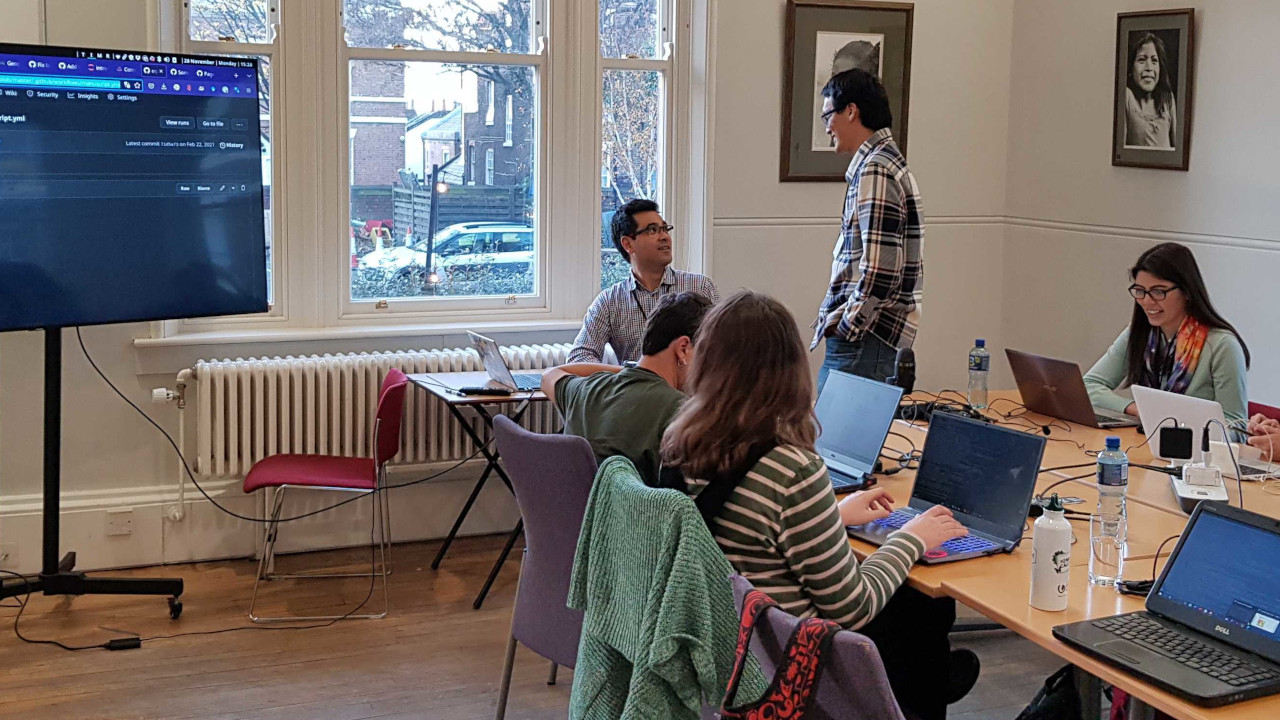
\includegraphics[width=\textwidth]{images/geopluscode.jpg}
  \end{center}
  \caption{
    Foto do evento \textit{Geo+Code UK} que organizei com meu financiamento
    do \href{https://software.ac.uk/}{Software Sustainability Institute} em
    Novembro de 2022. Durante o evento, demos início à criação de um
    livro texto digital sobre geofísica aplicada que será desenvolvido
    conjuntamente por educadores de diversas instituições do Reino Unido e
    Irlanda.
  }
\end{figure}
\begin{summarybox}[frametitle=\faInfoCircle{}\quad Portfólio de produção em ciência aberta]
  \begin{fa-ul}
    \faGithub & GitHub: \url{https://github.com/leouieda}
      (código, material didático) \\
    \aiFigshare & figshare: \url{https://figshare.com/authors/Leonardo\_Uieda/97471}
      (dados, apresentações, material suplementar) \\
    \aiImpactstory & Impactstory: \url{https://impactstory.org/u/0000-0001-6123-9515}
      (análise contextual da produção aberta) \\
    \faYoutube & YouTube: \url{https://youtube.com/LeonardoUieda}
      (palestras, tutoriais, aulas)
  \end{fa-ul}
\end{summarybox}

Como eu abordo a pesquisa e ensino.
Computacional primeiro.
Reprodutibilidade.
Dados abertos e FAIR principles.

Os princípios de dados FAIR (\textit{Findable, Accessible, Interoperable,
Reusable}) foram estabelecidos em \citet{Wilkinson2016}.
SSI.
EarthArXiv.
Software Underground.
JOSS.
pyOpenSci.

\begin{subsummarybox}[frametitle=\faInfoCircle{}\quad Apresentações sobre ciência aberta]
  \begin{paperlist}
    2022 &
      \Me.
      Getting started with Open Science,
      \emph{SPIN SPIN-ITN: Seismological Parameters and Instrumentation}.
      \GitHub{leouieda/2022-05-06-spin-open-science}.
      \\
    2021 &
      \Me, \Santiago.
      Python-based workflows for small-to-medium sized data: what works, what
      doesn't, and what can be improved,
      \emph{AGU Fall Meeting}. \GitHub{compgeolab/agu2021}.
      \\
    ~ &
      \Me.
      Academia e software livre: Desafios e oportunidades no Brasil e no exterior,
      \emph{National Observatory's SEG and EAGE Student Chapter},
      Rio de Janeiro, Brazil.
      \GitHub{leouieda/2021-07-22-on}.
      \YouTube{r2x-DN6laj8}.
      \\
    2020 &
      \Me.
      Geophysical research powered by open-source,
      \emph{Christian Albrechts Universität zu Kiel},
      Kiel, Germany.
      \GitHub{leouieda/2020-07-01-kiel}.
      \\
    ~ &
      \Me.
      Geophysical research powered by open-source,
      \emph{Departamento de Geofísica, IAG, Universidade de São Paulo}.
      \GitHub{leouieda/2020-06-18-usp}.
      \YouTube{VqI8BX1Yg54}.
      \\
    ~ &
      \Me.
      Geophysical research powered by open-source,
      \emph{Technische Universität Bergakademie Freiberg}.
      \GitHub{leouieda/2020-06-04-freiberg}.
      \\
    ~ &
      \Me.
      Geophysical research powered by open-source,
      \emph{Geographic Data Science Lab, University of Liverpool}.
      \GitHub{leouieda/liverpool-gdsl-2020}.
      \\
    2019 &
      \Me.
      Building the foundations for open-source geophysics,
      \emph{University of Liverpool}.
      \DOI{10.6084/m9.figshare.10255832}.
      \\
    2017 &
      \Me, \Paul.
      Nurturing reliable and robust open-source scientific software,
      \emph{AGU Fall Meeting}.
      \YouTube{0GO4ZZ5Ry6M}.
  \end{paperlist}
\end{subsummarybox}

Materiais de ensino aberto. Citar uns artigos aqui.

Listar aqui algumas das produções que são meio aleatórias, tipo o curso de
ciência aberta.

\section{Software livre}

Meu primeiro contato com a ciência aberta foi pesquisando sobre os sistemas
GNU/Linux que era operados pelo IAG.
Os princípios de software livre formaram o arcabouço da minha abordagem
científica.
Os códigos que possibilitam minhas atividades de pesquisa e ensino.

Apresento abaixo um resumo da minha produção relacionada a software livre,
seguido de contextualizações para cada um projetos relacionados a esse tema.

\subsection{Tesseroids}
\label{sec_tesseroids}

\begin{summarybox}[frametitle=\faInfoCircle{}\quad Informações sobre o projeto]
  \begin{fa-ul}
    \faLink & Página principal: \url{https://tesseroids.leouieda.com}
    \\
    \faGithub & Código: \url{https://github.com/leouieda/tesseroids}
    \\
    \faGavel & Licença: \href{https://github.com/leouieda/tesseroids/blob/master/LICENSE.txt}{BSD 3-clause}
    \\
    \aiGoogleScholarSquare & 146 citações no \href{https://scholar.google.com/citations?view\_op=view\_citation\&hl=en\&user=qfmPrUEAAAAJ\&citation\_for\_view=qfmPrUEAAAAJ:AXPGKjj\_ei8C}{Google Scholar}\footnotemark{} (acessado em 27/12/2022)
  \end{fa-ul}
\end{summarybox}
\footnotetext{Citações ao trabalho \citet{Uieda2016}.}
\begin{subsummarybox}[frametitle=\faFilePdf{}\quad Artigos publicados]
  \begin{paperlist}
    2016 &
      \Me, \Val, \Carla.
      Tesseroids: Forward modeling gravitational fields in spherical coordinates,
      \emph{Geophysics}, \DOI{10.1190/geo2015-0204.1}.
      \GitHub{pinga-lab/paper-tesseroids}.
  \end{paperlist}
\end{subsummarybox}

Figura com o logo do Tesseroids.
Primeiro projeto de software.
Como foi abordado.
Começou em C.
Passei para Python.
Voltei para C com a Carla em Trieste.
Uso do software e citações.

\subsection{Fatiando a Terra}
\label{sec_fatiando}

\begin{summarybox}[frametitle=\faInfoCircle{}\quad Informações sobre o projeto]
  \begin{fa-ul}
    \faLink & Página principal: \url{https://www.fatiando.org}
    \\
    \faGithub & Código: \url{https://github.com/fatiando}
    \\
    \faGavel & Licença: \href{https://opensource.org/licenses/BSD-3-Clause}{BSD 3-clause}
    \\
    \aiGoogleScholarSquare & 119 citações no \href{https://scholar.google.com/citations?user=qfmPrUEAAAAJ}{Google Scholar}\footnotemark{} (acessado em 27/12/2022)
  \end{fa-ul}
\end{summarybox}
\footnotetext{Total de citações aos trabalhos \citet{Uieda2013}, \citet{Uieda2018} e \citet{Uieda2020}.}
\begin{subsummarybox}[frametitle=\faFilePdf{}\quad Artigos publicados]
  \begin{paperlist}
    2020 &
      \Me, \Santiago, \Remi, \Hugo, \MattTurk, \Shapero, \Anderson, \Leeman.
      Pooch: A friend to fetch your data files.
      \emph{Journal of Open Source Software}.
      \DOI{10.21105/joss.01943}.
      \GitHub{fatiando/pooch}.
      \\
    2018 &
      \Me. Verde: Processing and gridding spatial data using Green's functions.
      \emph{Journal of Open Source Software}.
      \DOI{10.21105/joss.00957}.
      \GitHub{fatiando/verde}.
  \end{paperlist}
\end{subsummarybox}
\begin{subsummarybox}[frametitle=\faFile{}\quad Trabalhos completos em anais de eventos]
  \begin{paperlist}
    2013 &
      \Me, \Bi, \Val.
      Modeling the Earth with Fatiando a Terra,
      \emph{Proceedings of the 12th Python in Science Conference}.
      \DOI{10.25080/Majora-8b375195-010}.
      \GitHub{leouieda/scipy2013}.
  \end{paperlist}
\end{subsummarybox}
\begin{subsummarybox}[frametitle=\faInfoCircle{}\quad Outras apresentações]
  \begin{paperlist}
    2021 &
      \Me, \LLi, \Santiago, \Agustina.
      Design useful tools that do one thing well and work together: rediscovering
      the UNIX philosophy while building the Fatiando a Terra project,
      \emph{AGU Fall Meeting}.
      \GitHub{fatiando/agu2021}.
      \\
    ~ &
      \Me, \Santiago, \Agustina.
      Open-science for gravimetry: tools, challenges, and opportunities,
      \emph{GFZ Helmholtz Centre Potsdam}.
      \GitHub{leouieda/2021-06-22-gfz}.
      \YouTube{z-5dvWfB\_SM}.
      \\
    ~ &
      \Me, \Santiago, \Agustina.
      Fatiando a Terra: Open-source tools for geophysics,
      \emph{Geophysical Society of Houston}.
      \GitHub{fatiando/2021-gsh}.
      \\
    ~ &
      \Me, \Santiago, \Agustina, \LPerozzi, \MWieczorek.
      Harmonica and Boule: Modern Python tools for geophysical gravimetry,
      \emph{EGU General Assembly}.
      \DOI{10.5194/egusphere-egu21-8291}.
      \GitHub{fatiando/egu2021}.
      \\
    2015 &
      \Me.
      Fatiando a Terra: construindo uma base para ensino e pesquisa de geofísica,
      \emph{Universidade de São Paulo}.
      \DOI{10.6084/m9.figshare.1381870}
      \\
    2014 &
      \Me, \Bi, \Val.
      Using Fatiando a Terra to solve inverse problems in geophysics,
      \emph{Scipy}.
      \DOI{10.6084/m9.figshare.1089987}.
  \end{paperlist}
\end{subsummarybox}

Figura com o banner do Fatiando.

Como surgiu, o grupo no IAG, aprendendo subversion.
Colocar links para os commits.
Desenvolvimento na pós e o curso do IAG.
Uso na minha dissertação e tese e matérias da UERJ.

Entrada do Santiago como um marco.

Conhecendo o pessoal do SimPEG/PyGIMLi/GemPy e formação do Software Underground.
Overlap.
Reestruturação do Fatiando (link pro meu post).

Novos pacotes.
Mais participação consistente da comunidade (Agustina, Mariana, Lu, Matt).

Pooch como um caso de sucesso.
Como surgiu.
Podcast sobre o Pooch.
Uso em vários pacotes.

\subsection{Generic Mapping Tools}
\label{sec_gmt}

\begin{summarybox}[frametitle=\faInfoCircle{}\quad Informações sobre o projeto GMT]
  \begin{fa-ul}
    \faLink & Página principal: \url{https://www.generic-mapping-tools.org}
    \\
    \faGithub & Código: \url{https://github.com/GenericMappingTools}
    \\
    \faGavel & Licença: \href{https://opensource.org/licenses/LGPL-3.0}{GNU LGPL}
    \\
    \aiGoogleScholarSquare & 934 citações no \href{https://scholar.google.com/citations?view\_op=view\_citation\&hl=en\&user=qfmPrUEAAAAJ\&citation\_for\_view=qfmPrUEAAAAJ:hkOj\_22Ku90C}{Google Scholar}\footnotemark{} (acessado em 27/12/2022)
  \end{fa-ul}
\end{summarybox}
\footnotetext{Citações ao trabalho \citet{Wessel2019}.}
\begin{summarybox}[frametitle=\faInfoCircle{}\quad Informações sobre o projeto PyGMT]
  \begin{fa-ul}
    \faLink & Página principal: \url{https://www.pygmt.org}
    \\
    \faGithub & Código: \url{https://github.com/GenericMappingTools/pygmt}
    \\
    \faGavel & Licença: \href{https://github.com/GenericMappingTools/pygmt/blob/main/LICENSE.txt}{BSD 3-clause}
    \\
    \aiGoogleScholarSquare & 43 citações no \href{https://scholar.google.com/citations?view\_op=view\_citation\&hl=en\&user=qfmPrUEAAAAJ\&citation\_for\_view=qfmPrUEAAAAJ:-\_dYPAW6P2MC}{Google Scholar}\footnotemark{} (acessado em 27/12/2022)
  \end{fa-ul}
\end{summarybox}
\footnotetext{Citações ao trabalho \citet{Uieda2022}.}
\begin{subsummarybox}[frametitle=\faFilePdf{}\quad Artigos publicados]
  \begin{paperlist}
    2019 &
      \Paul, \Joaquim, \Me, \Remko, \Florian, \Walter, \Dongdong.
      The Generic Mapping Tools, Version 6.
      \emph{Geochemistry, Geophysics, Geosystems}.
      \DOI{10.1029/2019GC008515}.
  \end{paperlist}
\end{subsummarybox}
\begin{subsummarybox}[frametitle=\faInfoCircle{}\quad Apresentações]
  \begin{paperlist}
    2019 &
      \Me, \Paul.
      PyGMT: Accessing the Generic Mapping Tools from Python,
      \emph{AGU Fall Meeting}.
      \DOI{10.6084/m9.figshare.11320280}
      \\
    2018 &
      \Me, \Paul.
      Building an object-oriented Python interface for the Generic Mapping Tools,
      \emph{Scipy}.
      \DOI{10.6084/m9.figshare.6814052}
      \YouTube{6wMtfZXfTRM}
      \\
    ~ &
      \Me, \Paul.
      Integrating the Generic Mapping Tools with the Scientific Python Ecosystem,
      \emph{AOGS $15^{th}$ Annual Meeting}.
      \DOI{10.6084/m9.figshare.6399944}
      \\
    2017 &
      \Me, \Paul.
      A modern Python interface for the Generic Mapping Tools,
      \emph{AGU Fall Meeting}.
      \DOI{10.6084/m9.figshare.5662411}
      \\
    ~  &
      \Me, \Paul.
      Bringing the Generic Mapping Tools to Python,
      \emph{Scipy}.
      \DOI{10.6084/m9.figshare.7635833}
      \YouTube{93M4How7R24}
      \end{paperlist}
\end{subsummarybox}

Como me envolvi com o GMT.
Criação do PyGMT.
Comunidade que surgiu ao entrono.
Projeto da NSF e o Max.
\citep{Wessel2019}.

Summits do GMT.
Transição para o GitHub.
Website e documentação automatizados.
Abertura no modelo de desenvolvimento == maior participação tanto com exemplos,
discussões e até código.

\subsection{xlandsat}

\begin{summarybox}[frametitle=\faInfoCircle{}\quad Informações sobre o projeto]
  \begin{fa-ul}
    \faLink & Página principal: \url{https://compgeolab.org/xlandsat}
    \\
    \faGithub & Código: \url{https://github.com/compgeolab/xlandsat}
    \\
    \faGavel & Licença: \href{https://github.com/compgeolab/xlandsat/blob/main/LICENSE.txt}{MIT}
  \end{fa-ul}
\end{summarybox}

Último pacote a ser criado no âmbito do CompGeoLab.
Uso nas aulas e também para divulgação científica.
Por exemplo o Mauna Loa.
Colocar figura bonita e link para o meu blog.


\section{Dados abertos}

Na verdade melhor falar em FAIR.
Por que usar CC-BY ou CC0 é importante.

Compilação de dados do Fatiando.
Compilação da Austrália.


\section{Reprodutibilidade}

Alguma coisa sobre o Clarebout e Madagascar como influências iniciais.
Por que isso importa.
Lorena Barba.

Publicação de todo o código no GitHub e figshare desde meu primeiro artigo em
2012.
O approach atual de colocar o máximo possível nos pacotes durante o
desenvolvimento da pesquisa.
Exemplo da EQLGB.

\section{Acesso livre}

JOSS e EarthArXiv.


\section{Recursos educacionais abertos}

\begin{subsummarybox}[frametitle=\faFilePdf{}\quad Artigos publicados em revistas]
  \begin{paperlist}
    2017 &
      \Me.
      Step-by-step NMO correction,
      \emph{The Leading Edge},
      \DOI{10.1190/tle36020179.1}.
      \GitHub{pinga-lab/nmo-tutorial}.
      \\
    2014 &
      \Me, \Bi, \Val.
      Geophysical tutorial: Euler deconvolution of potential-field data,
      \emph{The Leading Edge},
      \DOI{10.1190/tle33040448.1}.
      \GitHub{pinga-lab/paper-tle-euler-tutorial}.
  \end{paperlist}
\end{subsummarybox}
\begin{subsummarybox}[frametitle=\faInfoCircle{}\quad Recursos educacionais]
  \begin{paperlist}
    2021 &
      \Me. A quick introduction to machine learning.
      \GitHub{leouieda/ml-intro}.
      \\
    2020 &
      \Me. Introduction to lithosphere dynamics.
      \GitHub{leouieda/lithosphere}.
      \\
    2020 &
      \Me. Introduction to remote sensing.
      \GitHub{leouieda/remote-sensing}.
      \\
    2015 &
      \Me. Matemática Especial 1: Introdução à computação e métodos numéricos.
      \GitHub{mat-esp/about}.
      \\
    2015 &
      \Me. Geofísica 2: Sismologia e métodos eletromagnéticos.
      \GitHub{leouieda/geofisica2}.
      \\
    2015 &
      \Me. Geofísica 1: Gravimetria e magnetometria.
      \GitHub{leouieda/geofisica1}.
      \\
    2014 &
      \Bi, \Me. Tópicos de inversão em geofísica.
      \DOI{10.6084/m9.figshare.1192984}.
      \GitHub{pinga-lab/inverse-problems}.
  \end{paperlist}
\end{subsummarybox}
\begin{subsummarybox}[frametitle=\faInfoCircle{}\quad Vídeos]
  \begin{paperlist}
    2022 & A geophysical tour of mid-ocean ridges. \YouTube{NzJmRlJCNbQ}
      \\
    2022 & Anatomy of a PyGMT figure. \YouTube{96\_reU\_yh5I}
      \\
    2021 & Downloading Landsat 8 images from USGS EarthExplorer. \YouTube{Wn\_G4fvitV8}
      \\
    2021 & Searching on Google for openly licensed images. \YouTube{ISu51NB5Z28}
      \\
    2020 & From scattered data to gridded products using Verde. \YouTube{-xZdNdvzm3E}
  \end{paperlist}
\end{subsummarybox}


https://www.unesco.org/en/open-educational-resources

Tutoriais da TLE.
Material de geofísica 1 e 2.
Material de Liverpool.

Geophysics Library e Geo+Code.



%==============================================================================
\chapter{Linhas de Pesquisa}
\label{cap_pesquisa}

\begin{figure}[h]
  \HeroFigPad
  \begin{center}
    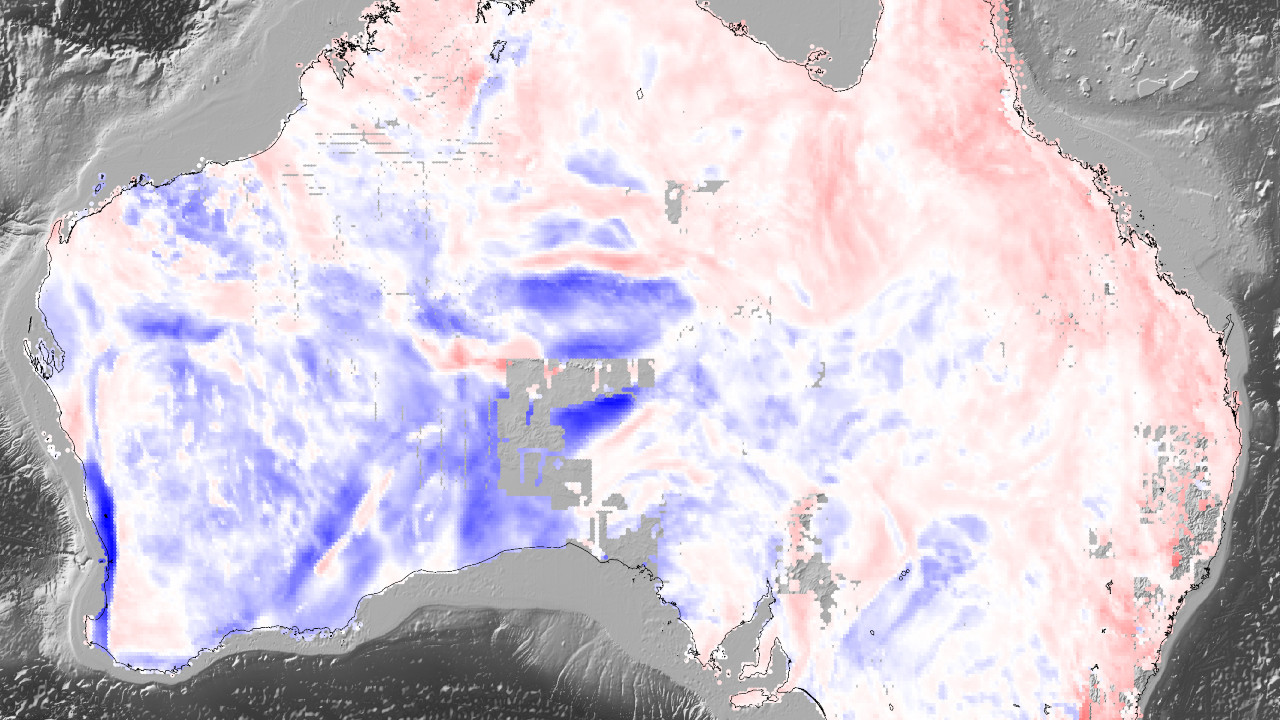
\includegraphics[width=\textwidth]{images/australia-ground-gravity-disturbance.jpg}
  \end{center}
  \caption{
    Compilação de dados terrestres de distúrbio da gravidade da Austrália.
    Distribuídos originalmente por \citet{Wynne2018}. Compilados e padronizados
    por \citet{Uieda2021} para facilitar o seu uso em diversas linhas de
    pesquisa.
  }
\end{figure}
\begin{summarybox}[frametitle=\faInfoCircle{}\quad Resumo das atividades]
  \begin{fa-ul}
    \faSearchDollar & Projetos financiados pelas agências: National Science
      Foundation (E.U.A.), Royal Society (Reino Unido) e Software Sustainability
      Institute (Reino Unido)\\
    \faUserGraduate & Orientações concluídas: 11 de graduação, 1 de mestrado, 1
      co-orientação de doutorado \\
    \faUser & Orientações em andamento: 1 de graduação, 1 de doutorado, 1
      co-orientação de doutorado \\
    \faFilePdf & 13 artigos publicados em revistas indexadas, 3 em outras
    revistas, 11 trabalhos completos em anais de eventos\footnotemark[1] \\
    \faComment & 38 apresentações de trabalho, sendo 13 dessas convidadas\footnotemark[1] \\
    \aiGoogleScholarSquare & 1736 citações no \href{https://scholar.google.com/citations?user=qfmPrUEAAAAJ}{Google Scholar} e 959 no \href{https://www.webofscience.com/wos/author/record/1766625}{Web of Science} (acessados em 27/12/2022)
  \end{fa-ul}
\end{summarybox}
\footnotetext[1]{O número de total trabalhos e apresentações pode ser diferente
das quantidades listadas abaixo. Alguns trabalhos e apresentações estão
listados em outras áreas de atuação (e.g., capítulo \ref{cap_cienciaaberta}) ou
pertencem a mais de uma linha de pesquisa.}

Esse capítulo é uma reflexão da minha trajetória de pesquisa, da graduação até
minha posição atual na Universidade de Liverpool.
Ciência de impacto.
Bem social.
Grandes problemas e questões.

É preciso enfatizar que nem todos os artigos, projetos financiados e
apresentações contados acima estão listados nas seções abaixo.
Alguns estão listados no capítulo \ref{cap_cienciaaberta}.

PINGA e CompGeoLab.

\section{Modelagem direta de campos gravitacionais em coordenadas esféricas}
\label{sec_modelagemdireta}

Tesseroids.
Ajuda da Wild-Pfeiffer.
TCC.
Carla.
Trieste.
Discretização adaptative.
Software.
Utilização para fazer os grids do GOCE.

Projeto inicial do Santiago.
Contato com Guangdong depois de uma revisão.
Mustafa começou com a parte elipsoidal.

\begin{subsummarybox}[frametitle=\faFilePdf{}\quad Artigos publicados]
  \begin{paperlist}
    2019 & \Santiago, \Agustina, \Gimenez, \Me.
      Gravitational field calculation in spherical coordinates using variable
      densities in depth.
      \emph{Geophysical Journal International}.
      \DOI{10.1093/gji/ggz277}.
      \GitHub{pinga-lab/tesseroid-variable-density}.
      \Preprint{10.31223/osf.io/3548g}.
      \Data{10.6084/m9.figshare.8239622}.
      \\
    ~ & \Guangdong, \Bo, \Me, \JLiu, \MKaban, \LChen, \RGuo.
      Efficient 3D large-scale forward-modeling and inversion of gravitational fields in
      spherical coordinates with application to lunar mascons.
      \emph{Journal of Geophysical Research: Solid Earth}.
      \DOI{10.1029/2019jb017691}.
      \Preprint{10.31223/osf.io/dzf9j}.
      \Data{10.6084/m9.figshare.7300523}.
      \\
    2016 & \Me, \Val, \Carla.
      Tesseroids: Forward modeling gravitational fields in spherical coordinates,
      \emph{Geophysics}, \DOI{10.1190/geo2015-0204.1}.
      \GitHub{pinga-lab/paper-tesseroids}.
  \end{paperlist}
\end{subsummarybox}
\begin{subsummarybox}[frametitle=\faFile{}\quad Trabalhos completos em anais de eventos]
  \begin{paperlist}
    2011 & \Me, \Everton, \Carla, \Eder.
      Optimal forward calculation method of the Marussi tensor due to a geologic
      structure at GOCE height,
      \emph{Proceedings of the 4th International GOCE User Workshop}.
      \DOI{10.6084/m9.figshare.92624}.
      \GitHub{leouieda/goce2011}.
  \end{paperlist}
\end{subsummarybox}
\begin{subsummarybox}[frametitle=\faInfoCircle{}\quad Outras apresentações]
  \begin{paperlist}
    2010 & \Me, \Naomi, \Carla.
      Computation of the gravity gradient tensor due to topographic masses
      using tesseroids,
      \emph{AGU Meeting of the Americas},
      Foz do Iguaçu, Brazil.
      \DOI{10.6084/m9.figshare.156858}
      \\
    2008 & \Me, \Naomi.
      Utilização de tesseróides na modelagem de dados de gradiometria
      gravimétrica,
      \emph{XIII Simpósio de Iniciação Científica do IAG-USP},
      São Paulo, Brazil.
      \DOI{10.6084/m9.figshare.4779760}
  \end{paperlist}
\end{subsummarybox}



\section{Inversão 3D em métodos potenciais}
\label{sec_planting}

Seed e trabalhos do Dio.
Inversão do Guangdong.

\begin{subsummarybox}[frametitle=\faFilePdf{}\quad Artigos publicados]
  \begin{paperlist}
    2019 &
      \Guangdong, \Bo, \Me, \JLiu, \MKaban, \LChen, \RGuo.
      Efficient 3D large-scale forward-modeling and inversion of gravitational fields in
      spherical coordinates with application to lunar mascons.
      \emph{Journal of Geophysical Research: Solid Earth}.
      \DOI{10.1029/2019jb017691}.
      \Preprint{10.31223/osf.io/dzf9j}.
      \Data{10.6084/m9.figshare.7300523}.
      \\
    2016 &
      \Dio, \Me, \Val.
      How two gravity-gradient inversion methods can be used to reveal different
      geologic features of ore deposit - A case study from the Quadrilátero
      Ferrífero (Brazil),
      \emph{Journal of Applied Geophysics},
      \DOI{10.1016/j.jappgeo.2016.04.011}.
      \\
    2014 &
      \Dio, \Me, \Val.
      Imaging iron ore from the Quadrilátero Ferrífero (Brazil) using geophysical
      inversion and drill hole data,
      \emph{Ore Geology Reviews},
      \DOI{10.1016/j.oregeorev.2014.02.011}.
      \\
    2012 &
      \Me, \Val.
      Robust 3D gravity gradient inversion by planting anomalous densities,
      \emph{Geophysics},
      \DOI{10.1190/geo2011-0388.1}.
      \GitHub{pinga-lab/paper-planting-densities}.
      \Data{10.6084/m9.figshare.91574}.
  \end{paperlist}
\end{subsummarybox}
\begin{subsummarybox}[frametitle=\faFile{}\quad Trabalhos completos em anais de eventos]
  \begin{paperlist}
    2012 &
      \Me, \Val.
      Use of the ``shape-of-anomaly'' data misfit in 3D inversion by planting
      anomalous densities,
      \emph{SEG Technical Program Expanded Abstracts},
      \DOI{10.1190/segam2012-0383.1}.
      \GitHub{leouieda/seg2012}.
      \\
    ~ &
      \Dio, \Me, \YLi, \Val, \BragaVale, \Angeli, \Peres.
      Iron ore interpretation using gravity-gradient inversions in the Carajás, Brazil.
      \emph{SEG Technical Program Expanded Abstracts},
      \DOI{10.1190/segam2012-0525.1}.
      \\
    2011 &
      \Me, \Val.
      Robust 3D gravity gradient inversion by planting anomalous densities,
      \emph{SEG Technical Program Expanded Abstracts},
      \DOI{10.1190/1.3628201}.
      \GitHub{leouieda/seg2011}
      \\
    ~ &
      \Me, \Val.
      3D gravity inversion by planting anomalous densities.
      \emph{12th International Congress of the Brazilian Geophysical Society},
      \DOI{10.1190/sbgf2011-179}.
      \GitHub{leouieda/sbgf2011}
      \\
    ~ &
      \Me, \Val.
      3D gravity gradient inversion by planting density anomalies.
      \emph{73th EAGE Conference and Exhibition incorporating SPE EUROPEC},
      \DOI{10.3997/2214-4609.20149567}.
      \GitHub{leouieda/eage2011}
      \\
    ~ &
      \Dio, \Me, \Val, \BragaVale, \Gomes.
      In-depth imaging of an iron orebody from Quadrilatero Ferrifero using 3D
      gravity gradient inversion,
      \emph{SEG Technical Program Expanded Abstracts},
      \DOI{10.1190/1.3628219}.
      \\
    ~ &
      \Dio, \Val, \Me, \BragaVale.
      Inversão de Dados de Aerogradiometria Gravimétrica 3D-FTG Aplicada a
      Exploração Mineral na Região do Quadrilátero Ferrífero,
      \emph{12th International Congress of the Brazilian Geophysical Society},
      \DOI{10.1190/sbgf2011-243}.
  \end{paperlist}
\end{subsummarybox}
\begin{subsummarybox}[frametitle=\faInfoCircle{}\quad Outras apresentações]
  \begin{paperlist}
  2014 &
  \Me, \Val.
  Gravity inversion in spherical coordinates using tesseroids,
  \emph{EGU General Assembly}.
  \DOI{10.6084/m9.figshare.1155457}
  \\
  2013 &
  \Me, \Val.
  3D magnetic inversion by planting anomalous densities,
  \emph{AGU Meeting of the Americas},
  Cancun, Mexico.
  \DOI{10.6084/m9.figshare.703651}
  \\
  2012 &
  \Me, \Val.
  Rapid 3D inversion of gravity and gravity gradient data to test geologic
  hypotheses,
  \emph{International Symposium on Gravity, Geoid and Height Systems},
  Venice, Italy.
  \DOI{10.6084/m9.figshare.156859}
  \end{paperlist}
\end{subsummarybox}


\begin{figure}[tb]
  \begin{center}
    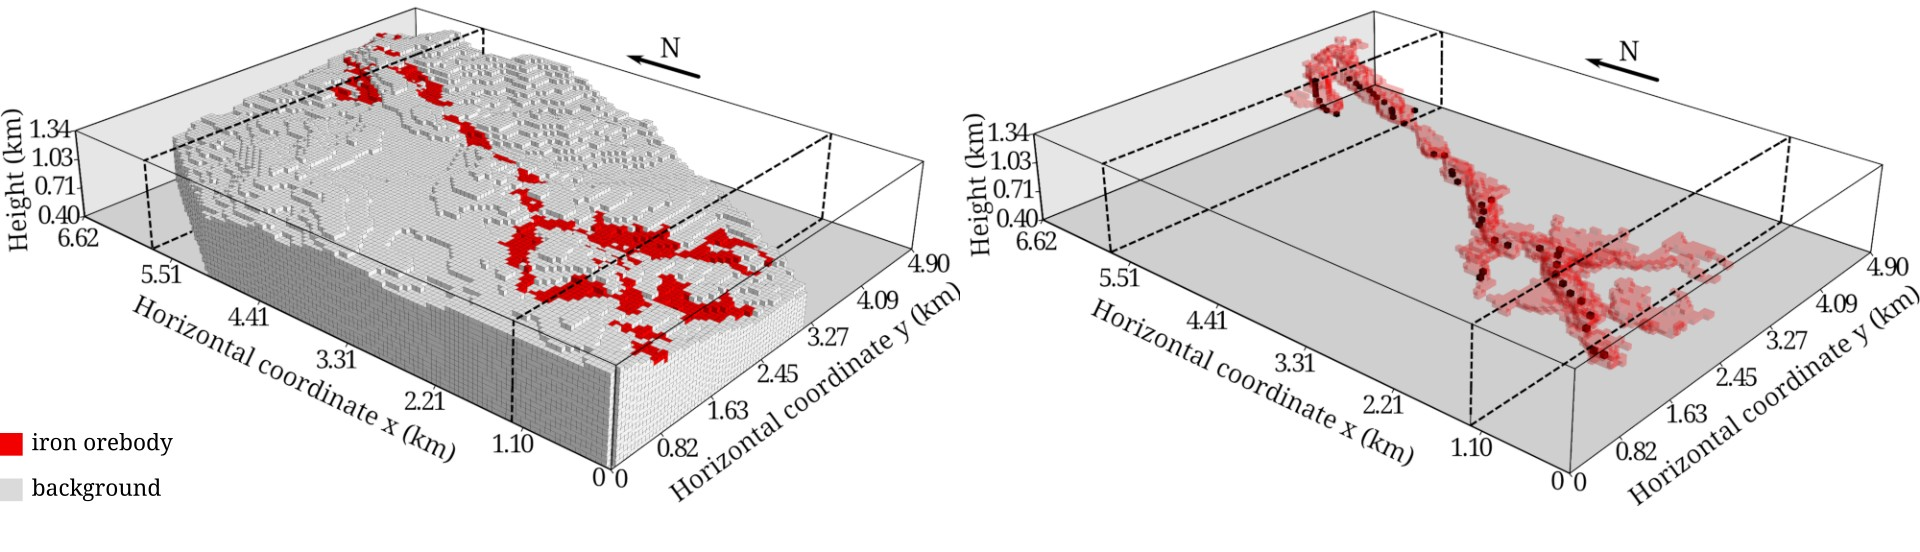
\includegraphics[width=\textwidth]{images/planting-results.jpg}
  \end{center}
  \caption{
    Modelo 3D gerado pela inversão de dados de gradiometria gravimétrica usando
    o algoritmo de plantação de \citet{Uieda2012}.
    Prismas vermelhos representam o itabirito da formação Cauê do Quadrilátero
    Ferrífero, prismas cinzas possuem contraste de densidade nulo e prismas
    pretos são as sementes utilizadas na inversão.
  }
  \label{fig_planting}
\end{figure}


\section{Determinação da espessura crustal através de distúrbios da gravidade}

Inversão Moho. Citações e utilização do software em outras áreas.
Listar todos os trabalho que estão usando o método.
Projeto do Aiden.

\begin{subsummarybox}[frametitle=\faFilePdf{}\quad Artigos publicados]
  \begin{paperlist}
    2017 &
      \Me, \Val.
      Fast non-linear gravity inversion in spherical coordinates with application
      to the South American Moho,
      \emph{Geophysical Journal International},
      \DOI{10.1093/gji/ggw390}.
      \Preprint{10.31223/osf.io/9ba4m}.
      \GitHub{pinga-lab/paper-moho-inversion-tesseroids}.
      \Data{10.6084/m9.figshare.3987267}.
  \end{paperlist}
\end{subsummarybox}
\begin{subsummarybox}[frametitle=\faInfoCircle{}\quad Apresentações]
  \begin{paperlist}
    2017 &
      \Me.
      Inverting gravity to map the Moho: A new method and the open source
      software that made it possible,
      \emph{Department of Geology and Geophysics, \UHM},
      Honolulu, USA.
      \DOI{10.6084/m9.figshare.4779766}
  \end{paperlist}
\end{subsummarybox}


\section{Camada equivalente para processamento de dados gravimétricos e magnetométricos}

PEL.
Gradient boosting.
Validação cruzada em blocos.
Trazendo coisas da aprendizagem de máquinas.

Projeto da India para juntar dados da Antártica.
Projeto do Hamed para juntar grav australia.
Projeto do Daniel.

\begin{subsummarybox}[frametitle=\faFilePdf{}\quad Artigos publicados]
  \begin{paperlist}
    2021 &
      \Santiago, \Me.
      Gradient-boosted equivalent sources.
      \emph{Geophysical Journal International}.
      \DOI{10.1093/gji/ggab297}.
      \GitHub{compgeolab/eql-gradient-boosted}.
      \Preprint{10.31223/X58G7C}.
      \Data{10.6084/m9.figshare.13604360}.
      \\
    2013 &
      \Bi, \Val, \Me.
      Polynomial equivalent layer,
      \emph{Geophysics},
      \DOI{10.1190/geo2012-0196.1}.
  \end{paperlist}
\end{subsummarybox}
\begin{subsummarybox}[frametitle=\faInfoCircle{}\quad Apresentações]
  \begin{paperlist}
    2020 &
      \Me, \Santiago.
      Evaluating the accuracy of equivalent-source predictions using
      cross-validation,
      \emph{EGU General Assembly}.
      \DOI{10.5194/egusphere-egu2020-15729}.
      \Data{10.6084/m9.figshare.12245372}
  \end{paperlist}
\end{subsummarybox}


\section{Deconvolução de Euler}

Trabalho do Felipe Melo.
Tutorial na TLE.
Projeto do Lottie.
Projeto do Gelson.

\begin{subsummarybox}[frametitle=\faFilePdf{}\quad Artigos publicados]
  \begin{paperlist}
    2014 &
      \Me, \Bi, \Val.
      Geophysical tutorial: Euler deconvolution of potential-field data,
      \emph{The Leading Edge},
      \DOI{10.1190/tle33040448.1}.
      \GitHub{pinga-lab/paper-tle-euler-tutorial}.
      \\
    2013 &
      \Figura, \Val, \Me, \Bi, \JB.
      Estimating the nature and the horizontal and vertical positions of 3D
      magnetic sources using Euler deconvolution,
      \emph{Geophysics},
      \DOI{10.1190/geo2012-0515.1}.
  \end{paperlist}
\end{subsummarybox}
\begin{subsummarybox}[frametitle=\faFile{}\quad Trabalhos completos em anais de eventos]
  \begin{paperlist}
    2014  &
      \Figura, \Val, \Me, \Bi, \JB.
      A Single Euler Solution Per Anomaly,
      \emph{76th EAGE Conference and Exhibition 2014},
      \DOI{10.3997/2214-4609.20140891}.
  \end{paperlist}
\end{subsummarybox}


\section{Interpolação de dados geofísicos}

\begin{subsummarybox}[frametitle=\faFilePdf{}\quad Artigos publicados]
  \begin{paperlist}
    2018 &
      \Me.
      Verde: Processing and gridding spatial data using Green's functions.
      \emph{Journal of Open Source Software}.
      \DOI{10.21105/joss.00957}.
      \GitHub{fatiando/verde}.
  \end{paperlist}
\end{subsummarybox}
\begin{subsummarybox}[frametitle=\faInfoCircle{}\quad Apresentações]
  \begin{paperlist}
    2018 &
      \Me, \Eric, \Paul, \David.
      Coupled Interpolation of Three-component GPS Velocities,
      \emph{AGU Fall Meeting}.
      \DOI{10.6084/m9.figshare.7440683}
      \\
    ~ &
      \Me, \David, \Paul.
      Joint Interpolation of 3-component GPS Velocities Constrained by
      Elasticity,
      \emph{AOGS $15^{th}$ Annual Meeting}.
      \DOI{10.6084/m9.figshare.6387467}
  \end{paperlist}
\end{subsummarybox}

Verde e interpolação de GPS com o Sandwell.
Trabalhos do Majed e Sarah.

\section{Modelagem de dados de microscopia magnética}
\label{sec_micromag}

Projeto do Gelson.
Junta com o paper da Dai (colocar aqui).
Financiamento da Royal Society.
Voltando à paleomag depois da primeira IC.

\begin{subsummarybox}[frametitle=\faFilePdf{}\quad Artigos publicados]
  \begin{paperlist}
    2015 &
      \Bi, \Dai, \Val, \Me.
      Estimation of the total magnetization direction of approximately spherical
      bodies,
      \emph{Nonlinear Processes in Geophysics},
      \DOI{10.5194/npg-22-215-2015}.
      \GitHub{pinga-lab/Total-magnetization-of-spherical-bodies}.
  \end{paperlist}
\end{subsummarybox}


\section{Determinação do fluxo geotermal Antártico através de dados magnetométricos}

Projeto da India que tá começando junto com o Bi.
Colaboração com o pessoal da BAS e o Lu Li.
Usar a compilação de dados produzida com camada equivalente para fazer uma
inversão usando tesseroides.


%==============================================================================
\chapter{Experiência em Ensino}
\label{cap_ensino}

\begin{figure}[h]
  \HeroFigPad
  \begin{center}
    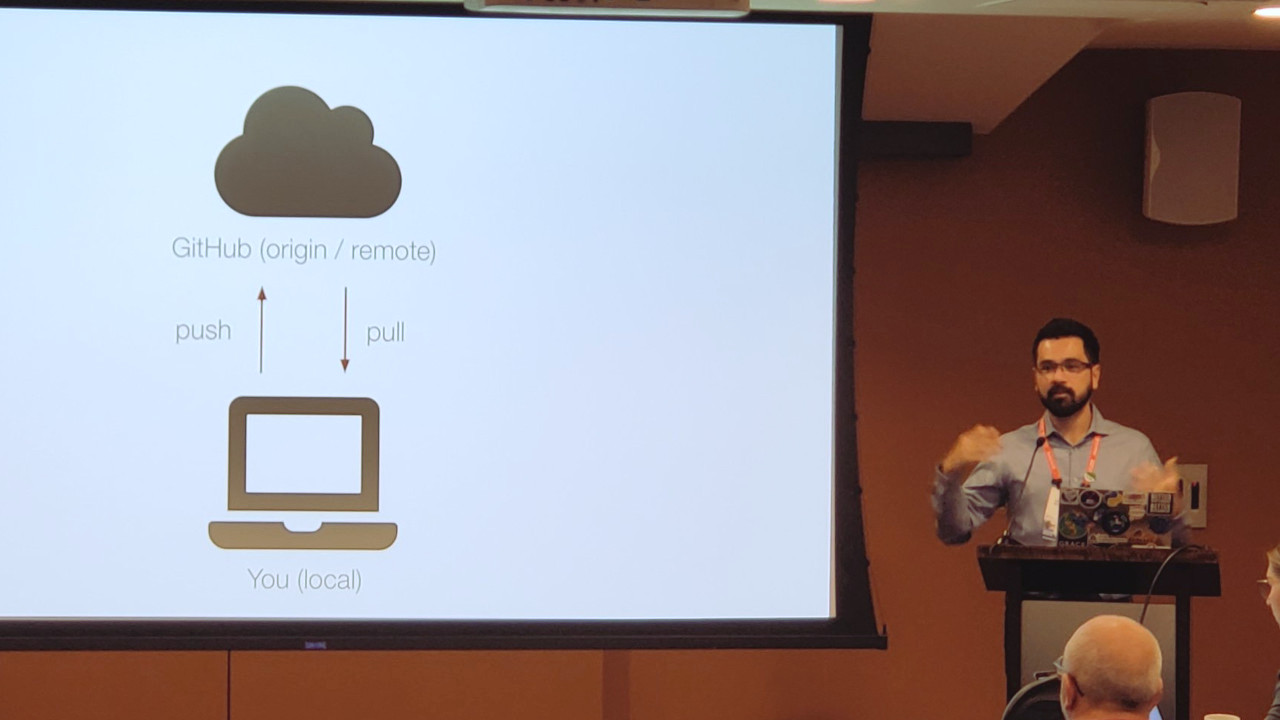
\includegraphics[width=\textwidth]{images/agu-2019-git-lesson.jpg}
  \end{center}
  \caption{
    Foto tirada durante o curso ``Best Practices for Developing and Sustaining
    Your Open-Source Research Software'' que ministrei em 2019 durante o
    \href{https://github.com/agu-ossi/2019-agu-oss}{AGU Fall Meeting} em
    São Francisco, E.U.A.
  }
\end{figure}
\begin{summarybox}[frametitle=\faChalkboardTeacher{}\quad Resumo da experiência de ensino]
  \begin{fa-ul}
    \faChalkboardTeacher & 10 disciplinas de graduação ministradas \\
    \faClock & 17 cursos de curta duração ministrados internacionalmente \\
    \faCheckSquare & Habilitação em pedagogia e técnicas de ensino aplicadas ao
      ensino superior \\
    \faLightbulb & Tópicos ensinados incluem: gravimetria, magnetometria,
    sismologia, sensoriamento remoto, métodos numéricos, programação em Python,
    métodos de campo em geofísica, introdução à geologia, problemas inversos,
    geofísica global e geodinâmica da litosfera.
  \end{fa-ul}
\end{summarybox}

Ensino é a parte que eu mais gosto.
Como eu abordo o ensino.
Citar artigos de pedagogia.
Figura do notebook de ondas sísmicas.
Ensino guiando a pesquisa (imagem do Havaí e trabalho do Gelson).

Crise na geociências.
Fenômeno global citar trabalhos nos EUA e Inglaterra.
Qual é o papel da geofísica além do petróleo.
Ciência de dados.
Aplicações ambientais.
Importância de conceitos de programação para ser cidadão informado no século XXI.

\section{Cursos de curta duração}
\label{sec_workshops}

\begin{subsummarybox}[frametitle=\faClock{}\quad Cursos e workshops ministrados]
  \begin{paperlist}
    2022 &
      Crafting beautiful maps with PyGMT.
      \textit{EGU General Assembly}.
      \GitHub{GenericMappingTools/egu22pygmt}
      \\
    ~ &
      A geophysical tour of mid-ocean ridges.
      \textit{Transform 2022} (online).
      \GitHub{leouieda/transform2022}.
      \YouTube{NzJmRlJCNbQ}
      \\
    2021 &
      The Generic Mapping Tools for Geodesy.
      \textit{UNAVCO} (online).
      \GitHub{GenericMappingTools/2021-unavco-course}
      \\
    2020 &
      Let's build a geophysical inversion with Python.
      \textit{IRTG-2379 Graduate School: Modern Inverse Problems},
      \textit{RWTH Aachen University} (online).
      \GitHub{compgeolab/2020-aachen-inverse-problems}
      \\
    ~ &
      The Generic Mapping Tools for Geodesy.
      \textit{UNAVCO} (online).
      \GitHub{GenericMappingTools/2020-unavco-course}.
      \YouTube{EQgxDmCXvj4}
      \\
    ~  &
      From scattered data to gridded products using Verde.
      \textit{Transform 2020} (online).
      \GitHub{fatiando/transform2020}.
      \YouTube{-xZdNdvzm3E}
      \\
    2019 &
      Best Practices for Developing and Sustaining Your Open-Source Research Software.
      \textit{AGU Fall Meeting}.
      \GitHub{agu-ossi/2019-agu-oss}
      \\
    ~  &
      Become a Generic Mapping Tools Contributor Even If You Can't Code.
      \textit{AGU Fall Meeting}
      \\
    ~  &
      The Generic Mapping Tools for Geodesy.
      \textit{Scripps Institution of Oceanography} and \textit{UNAVCO}.
      \GitHub{GenericMappingTools/2019-unavco-course}.
      \YouTube{uPUt4\_kd6m8}
      \\
    ~  &
      Introduction to Python Workshop (Earth Sciences REU program).
      \textit{Department of Geology and Geophysics, \UHM}.
      \GitHub{leouieda/2019-06-reu-python}
      \\
    2018 &
      Best Practices for Modern Open-Source Research Codes.
      \textit{AGU Fall Meeting}.
      \GitHub{agu-ossi/2018-agu-oss}
      \\
    ~  &
      Git and GitHub: What are their uses? Are they worth the effort? Let's find out!
      \textit{ASPRS UHM Student Chapter, \UHM}
      \\
    2017 &
      Introduction to Python.
      \textit{Department of Geology and Geophysics, \UHM}.
      \GitHub{leouieda/python-hawaii-2017}
      \\
    2016 &
      Python for Geologists (SAGEO).
      \textit{Faculdade de Geologia, \UERJ}.
      \GitHub{leouieda/python-geologia-2016}
      \\
    ~  &
      Python como uma ferramenta numérica em Ciências da Terra: uma nova
      abordagem de programação.
      \textit{XVIII Escola de Verão de Geofísica do IAG-USP}.
      \GitHub{leouieda/verao2016}
      \\
    2014 &
      Tópicos de inversão em geofísica.
      \textit{III Semana de Geofísica da UnB}.
      \GitHub{pinga-lab/inversao-unb-2014}
      \\
    2012 &
      Tópicos de inversão em geofísica.
      \textit{XVI Escola de Verão de Geofísica do IAG-USP}.
      \GitHub{pinga-lab/inversao-iag-2012}
  \end{paperlist}
\end{subsummarybox}

Primeira experiência na USP.
Escolas de verão no Brasil.
Software Carpentry.
AGU.
GMT e GMTSAR.
Transform.

\section{Disciplinas de graduação}

\begin{subsummarybox}[frametitle=\faClock{}\quad Disciplinas ministradas]
  \begin{courselist}
    2023--atual  &
      ENVS219: Earth and Environmental Data Science (\textit{em
      desenvolvimento}).
      \textit{University of Liverpool}.
      \\
    2020--atual  &
      ENVS398: Global Geophysics and Geodynamics.
      \textit{University of Liverpool}.
      \GitHub{leouieda/lithosphere}
      \\
    ~ &
    ENVS258: Environmental Geophysics.
      \textit{University of Liverpool}.
      \GitHub{leouieda/remote-sensing}.
      \GitHub{leouieda/gravity-processing}.
      \\
    ~ &
    ENVS386: Geophysical Data Modelling.
      \textit{University of Liverpool}.
      \GitHub{leouieda/ml-intro}.
      \\
    ~ &
      ENVS101/106: Study Skills and GIS (tutorial).
      \textit{University of Liverpool}.
      \\
    2019--2021 &
      ENVS123: Introduction to Geoscience and Earth History.
      \textit{University of Liverpool}.
      \\
    2019--2020  &
      ENVS363: Geophysics Field School.
      \textit{University of Liverpool}.
      \\
    2015--2016 &
      IME03-1366 Matemática Especial I. \textit{\UERJ}.
      \GitHub{mat-esp/about}
      \\
    2014--2016 &
      FGEL04-12422 Geofísica II. \textit{\UERJ}.
      \GitHub{leouieda/geofisica2}
      \\
    ~ &
      FGEL04-12421 Geofísica I. \textit{\UERJ}.
      \GitHub{leouieda/geofisica1}
      \\
    2015 &
      FGEL01-00805 Geologia Geral I. \textit{\UERJ}.
  \end{courselist}
\end{subsummarybox}

\subsection{\UERJ{}}
\label{sec_ensino_uerj}

\subsection{University of Liverpool}
\label{sec_ensino_liverpool}

Matérias que eu criei.
Material didático.
Paraninfo da turma.
Disciplinas de campo.

PGCAP.
Disciplinas de campo.
Matérias criadas em Liverpool.
Machine learning.
Environmental Data Science em todos os cursos.
Coordenação do curso.


%==============================================================================
\chapter{Atividades de Extensão}
\label{cap_extensao}

Entrevistas nos podcasts, open days.
Parte que está faltando mais e que eu quero investir mais tempo.
Pandemia significou que muitas dessas atividades não estavam acontecendo antes.
Experimento com o imã e Phyphox.


%==============================================================================
\chapter{Conclusão}
\label{cap_conclusao}

Repete resumo dos principais pontos.
Termina com o que eu pretendo conquistar no futuro.

Incluir resumo de ideias de pesquisa (fazer referência ao projeto),
extensão (cursos de programação, videos sobre geofísica) e ensino (introduzir
computação ao longo do currículo, software carpentry no verão, livros abertos,
mesa redonda do futuro da geofísica).

%==============================================================================
\backmatter
\bibliographystyle{apalike-doi}
\bibliography{references}

\end{document}
